%%%%%%%%%%%%%%%%%%%%%%%%%%%%%%%%%%%%%%%%%%%%%%%%%% %%%%%%%%%%%%%%%%%%%%%%%%%%%%%%%%
% Content: The main file of the diploma thesis template (master's/engineering).
% Prepared by: Tomasz Kubik <tomasz.kubik@pwr.edu.pl>
% Date: January 2023
% Version: 0.9
% Requirements: pdflatex compiler
%%%%%%%%%%%%%%%%%%%%%%%%%%%%%%%%%%%%%%%%%%%%%%%%%% %%%%%%%%%%%%%%%%%%%%%%%%%%%%%%%%

\documentclass[a4paper,onecolumn,oneside,12pt,extrafontsizes]{memoir}
% To prepare a printout for the archive, you can:
% a) prepare a PDF in which two pages will be inserted on one physical page and print such a document on both sides (recommended approach)
%
% Such a document can be prepared via:
% - printout from Adobe Acrobat Reader with the "Multiple" option - "Page size and handling" section
% - use of psutils tools
%
% Windows (assuming the MiKTeX distribution includes the miktex-psutils-bin-x64-2.9 package):
% "c:\Program Files\MiKTeX 2.9\miktex\bin\x64\pdf2ps.exe" Dyplom.pdf Dyplom.ps
% "c:\Program Files\MiKTeX 2.9\miktex\bin\x64\psnup.exe" -2 Dyplom.ps Dyplom2.ps
% "c:\Program Files\MiKTeX 2.9\miktex\bin\x64\ps2pdf.exe" Dyplom2.ps Dyplom2.pdf
% Del Dyplom2.ps Dyplom.ps
%
% Linux:
% pdf2ps Diplom.pdf - | psnup -2 | ps2pdf - Diplom2.pdf
%
% b) recompile the document by reducing the font size (this approach is not recommended because it changes the formatting of the document)
%
% To do this, just use the following commands (instead of documentclass from the first line):
% \documentclass[a4paper,onecolumn,twoside,10pt]{memoir}
% \renewcommand{\normalsize}{\fontsize{8pt}{10pt}\selectfont}

%\usepackage[cp1250]{inputenc} % Please leave if the encoding of the edited files is cp1250
\usepackage[utf8]{inputenc} % Please use instead of above if the encoding of the files you are editing is UTF8
\usepackage[T1]{fontenc}
\usepackage[polish,english]{babel} % The order of attributes is important here (for work in Polish, Polish should be at the end)
%\DisemulatePackage{setspace}
\usepackage{setspace}
\usepackage{color,calc}
%\usepackage{soul} % package with commands for underlining, underlining, highlighting text (rather unnecessary)
\usepackage{ebgaramond} % garamond font package, needed only for the title page, must appear before the tgtermes package

%% To obtain Polish letters in PDF (and not conglomerates) we use the tgterms font package.
%% This package defines Times font clones with the following shapes: normal, bold, italic, bold italic.
%% This package is missing a slanted font (similar to Italic).
%% If the slanted font is used anywhere in the document (e.g. after using the \textsl{} command), then
%% latex will substitute the standard font and report this in a warning.
%% Also, tgtermes is a font for the text. Any mathematical formulas will be formatted in the default formula font.
%% If patterns are to be formatted with different fonts, this must be explicitly declared.

%% After installing the tgtermes package, you may need to update the information
%% about available fonts and maps. You can do this from the console (as administrator)
%% initexmf --admin --update-fndb
%% initexmf --admin --mkmaps

\usepackage{tgtermes}   
\renewcommand*\ttdefault{txtt}


%%%%%%%%%%%%%%%%%%%%%%%%%%%%%%%%%%%%%%%%%%%%%%%%%% %%%%%%%%%%%%%%%%%%%%%%%%%%%%%%%%
%% Settings responsible for the way the document is broken
%% and arrangement of floating elements
%%%%%%%%%%%%%%%%%%%%%%%%%%%%%%%%%%%%%%%%%%%%%%%%%% %%%%%%%%%%%%%%%%%%%%%%%%%%%%%%%%
%\hyphenpenalty=10000 % don't hyphenate words too often
\clubpenalty=10000      % penalty for orphans
\widowpenalty=10000     % don't leave widows
%\brokenpenalty=10000 % do not break words between pages - you had to turn it off because it did not break lines in lstlisting
%\exhyphenpenalty=999999 % don't share lines with hyphen - you had to turn it off because it didn't break lines in lstlisting
\righthyphenmin=3			  % divide at least 3 letters

%\tolerance=4500
%\pretolerance=250
%\hfuzz=1.5pt
%\hbadness=1450

\renewcommand{\topfraction}{0.95}
\renewcommand{\bottomfraction}{0.95}
\renewcommand{\textfraction}{0.05}
\renewcommand{\floatpagefraction}{0.35}

%%%%%%%%%%%%%%%%%%%%%%%%%%%%%%%%%%%%%%%%%%%%%%%%%% %%%%%%%%%%%%%%%%%%%%%%%%%%%%%%%%
%% Size settings: text, header and footer, margins
%% for memoir class documents
%%%%%%%%%%%%%%%%%%%%%%%%%%%%%%%%%%%%%%%%%%%%%%%%%% %%%%%%%%%%%%%%%%%%%%%%%%%%%%%%%%
\setlength{\headsep}{10pt} 
\setlength{\headheight}{15pt} % baselineskip value for 11pt font i.e. \small is 13.6pt
\setlength{\footskip}{\headsep+\headheight}
\setlength{\uppermargin}{\headheight+\headsep+1cm}
\setlength{\textheight}{\paperheight-\uppermargin-\footskip-1.5cm}
\setlength{\textwidth}{\paperwidth-5cm}
\setlength{\spinemargin}{2.5cm}
\setlength{\foremargin}{2.5cm}
\setlength{\marginparsep}{2mm}
\setlength{\marginparwidth}{2.3mm}
%\settrimmedsize{297mm}{210mm}{*}
%\settrims{0mm}{0mm}	
\checkandfixthelayout[fixed] % necessary to arrange everything correctly
%%%%%%%%%%%%%%%%%%%%%%%%%%%%%%%%%%%%%%%%%%%%%%%%%% %%%%%%%%%%%%%%%%%%%%%%%%%%%%%%%%
%% Line spacing, still, spacing settings
%%%%%%%%%%%%%%%%%%%%%%%%%%%%%%%%%%%%%%%%%%%%%%%%%% %%%%%%%%%%%%%%%%%%%%%%%%%%%%%%%%
\linespread{1}
%\linespread{1.241}
\setlength{\parindent}{14.5pt}


\usepackage{multicol} % a package that allows you to create multi-column text
%%%%%%%%%%%%%%%%%%%%%%%%%%%%%%%%%%%%%%%%%%%%%%%%%% %%%%%%%%%%%%%%%%%%%%%%%%%%%%%%%%
%% Table formatting packages
%%%%%%%%%%%%%%%%%%%%%%%%%%%%%%%%%%%%%%%%%%%%%%%%%% %%%%%%%%%%%%%%%%%%%%%%%%%%%%%%%%
\usepackage{tabularx}
% Please use tabularx only. Please do not use other packages!!!
% The document can certainly be edited without using them.
%\usepackage{longtable}
%\usepackage{ltxtable}
%\usepackage{tabulary}

%%%%%%%%%%%%%%%%%%%%%%%%%%%%%%%%%%%%%%%%%%%%%%%%%% %%%%%%%%%%%%%%%%%%%%%%%%%%%%%%%%
%% Package for inserting code snippets
%%%%%%%%%%%%%%%%%%%%%%%%%%%%%%%%%%%%%%%%%%%%%%%%%% %%%%%%%%%%%%%%%%%%%%%%%%%%%%%%%%
\usepackage{listings} 
\usepackage{xpatch}
\makeatletter
\xpatchcmd\l@lstlisting{1.5em}{0em}{}{}
\makeatother
% Package provides lstlisting environment. It is highly customizable.
% You can configure each listing individually or globally using the \lstset{} command.

% It is recommended that the source code be output using the \ttfamily typewriter font
% Because the source code, even when truncated to interesting parts, can be large, you should reduce the font size.
% \small (for short snippets) and \footnotesize (for longer snippets) are recommended.

% Additionally, you can declare the line numbering method during configuration. However, line numbering is recommended
% only in cases where there are some references to specific lines in the text being edited.
% If there are no such references, line numbering is unnecessary. Please do not use it then.
% When enabling line numbering, pay attention to where these numbers appear.
% Without changing additional parameters, they appear in the margin of the page (which is undesirable).

\lstset{
  basicstyle=\small\ttfamily, % or basicstyle=\footnotesize\ttfamily
  %%columns=fullflexible,
	%%showstringspaces=false,
	%%showspaces=false,
  breaklines=true,
  postbreak=\mbox{\textcolor{red}{$\hookrightarrow$}\space}, 
  %%numbers=left,  % this and the lines below concern the numbering setting and how it is output
  %%firstnumber=1, 
  %%numberfirstline=true, 
	%%xleftmargin=17pt,
  %%framexleftmargin=17pt,
  %%framexrightmargin=5pt,
  %%framexbottommargin=4pt,
	belowskip=.5\baselineskip,
	literate={\_}{{\_\allowbreak}}1 % this declaration is useful if names containing underscores are to be escaped in the listing
	}
	
	% If the edited file is not in cp1250 encoding, there is a problem with Polish characters appearing in the inserted code.
	% Therefore, when working on files in UTF8 encoding, you need to declare the mapping as below (just unmark).
	% Unfortunately, when using this mapping, you may encounter problems with syntax highlighting (see below).
\lstset{literate=%-
{ą}{{\k{a}}}1 {ć}{{\'c}}1 {ę}{{\k{e}}}1 {ł}{{\l{}}}1 {ń}{{\'n}}1 {ó}{{\'o}}1 {ś}{{\'s}}1 {ż}{{\.z}}1 {ź}{{\'z}}1 {Ą}{{\k{A}}}1 {Ć}{{\'C}}1 {Ę}{{\k{E}}}1 {Ł}{{\L{}}}1 {Ń}{{\'N}}1 {Ó}{{\'O}}1 {Ś}{{\'S}}1 {Ż}{{\.Z}}1 {Ź}{{\'Z}}1 
    {Ö}{{\"O}}1
    {Ä}{{\"A}}1
    {Ü}{{\"U}}1
    {ß}{{\ss}}1
    {ü}{{\"u}}1
    {ä}{{\"a}}1
    {ö}{{\"o}}1
    {~}{{\textasciitilde}}1
		{—}{{{\textemdash} }}1
}%{\ \ }{{\ }}1}


%% lstlisting allows you to style syntax highlighting of selected languages.
%% This works by defining key words and how they are displayed.
%% Because this is a simple mechanism, it is sometimes difficult to achieve the results that IDE tools can provide.
%% However, in most cases the results achieved are satisfactory.


%% lstlisting supports several of the most popular languages by default.
%%\lstloadlanguages{% Check Documentation for further languages ...
%%C,
%%C++,
%%csh,
%%Java
%%}
%% Other languages must be defined. The following are examples of language and style definitions.

\definecolor{lightgray}{rgb}{.9,.9,.9}
\definecolor{darkgray}{rgb}{.4,.4,.4}
\definecolor{purple}{rgb}{0.65, 0.12, 0.82}
\definecolor{javared}{rgb}{0.6,0,0} % for strings
\definecolor{javagreen}{rgb}{0.25,0.5,0.35} % comments
\definecolor{javapurple}{rgb}{0.5,0,0.35} % keywords
\definecolor{javadocblue}{rgb}{0.25,0.35,0.75} % javadoc
 
\lstdefinelanguage{JavaScript}{ 
	keywords={typeof, new, true, false, catch, function, return, null, catch, switch, var, if, in, while, do, else, case, break},
	keywordstyle=\color{blue}\bfseries,
	ndkeywords={class, export, boolean, throw, implements, import, this},
	ndkeywordstyle=\color{darkgray}\bfseries,
	identifierstyle=\color{black},
	sensitive=false,
	comment=[l]{//},
	morecomment=[s]{/*}{*/},
	commentstyle=\color{purple}\ttfamily,
	stringstyle=\color{red}\ttfamily,
	morestring=[b]',
	morestring=[b]'
}
\lstdefinestyle{JavaScriptStyle}{
	language=JavaScript,
	commentstyle=\color{javagreen}, % unfortunately, if keywords appear in the comment line, they will be colored
	backgroundcolor=,%\color{lightgray}, % you can set a background color, but it is not recommended
	extendedchars=true,
	basicstyle=\footnotesize\ttfamily,
	showstringspaces=false,
	showspaces=false,
	numbers=none,%left,
	numberstyle=\footnotesize,
	numbersep=9pt,
	tabsize=2,
	breaklines=true,
	showtabs=false,
	captionpos=t
}

\lstdefinestyle{JavaStyle}{
basicstyle=\footnotesize\ttfamily,
keywordstyle=\color{javapurple}\bfseries,
stringstyle=\color{javared},
commentstyle=\color{javagreen},
morecomment=[s][\color{javadocblue}]{/**}{*/},
numbers=none,%left,
numberstyle=\tiny\color{black},
stepnumber=2,
numbersep=10pt,
tabsize=4,
showspaces=false,
showstringspaces=false,
captionpos=t
}

\definecolor{pblue}{rgb}{0.13,0.13,1}
\definecolor{pgreen}{rgb}{0,0.5,0}
\definecolor{pred}{rgb}{0.9,0,0}
\definecolor{pgrey}{rgb}{0.46,0.45,0.48}
\definecolor{dark-grey}{rgb}{0.4,0.4,0.4}
% styl json
\newcommand\JSONnumbervaluestyle{\color{blue}}
\newcommand\JSONstringvaluestyle{\color{red}}

\newif\ifcolonfoundonthisline

\makeatletter

\lstdefinestyle{json-style}  
{
	showstringspaces    = false,
	keywords            = {false,true},
	alsoletter          = 0123456789.,
	morestring          = [s]{"}{"},
	stringstyle         = \ifcolonfoundonthisline\JSONstringvaluestyle\fi,
	MoreSelectCharTable =%
	\lst@DefSaveDef{`:}\colon@json{\processColon@json},
	basicstyle          = \footnotesize\ttfamily,
	keywordstyle        = \ttfamily\bfseries,
	numbers				= left, % comment out if line numbering is unnecessary
	numberstyle={\footnotesize\ttfamily\color{dark-grey}},
	xleftmargin			= 2em % comment out if line numbering is unnecessary
}

\newcommand\processColon@json{%
	\colon@json%
	\ifnum\lst@mode=\lst@Pmode%
	\global\colonfoundonthislinetrue%
	\fi
}

\lst@AddToHook{Output}{%
	\ifcolonfoundonthisline%
	\ifnum\lst@mode=\lst@Pmode%
	\def\lst@thestyle{\JSONnumbervaluestyle}%
	\fi
	\fi
	\lsthk@DetectKeywords% 
}

\lst@AddToHook{EOL}%
{\global\colonfoundonthislinefalse}

\makeatother

%%\definecolor{red}{rgb}{0.6,0,0} % for strings
%%\definecolor{blue}{rgb}{0,0,0.6}
%%\definecolor{green}{rgb}{0,0.8,0}
%%\definecolor{cyan}{rgb}{0.0,0.6,0.6}
%%
%%\lstdefinestyle{sqlstyle}{
%%language=SQL,
%%basicstyle=\footnotesize\ttfamily, 
%%numbers=left, 
%%numberstyle=\tiny, 
%%numbersep=5pt, 
%%tabsize=2, 
%%extendedchars=true, 
%%breaklines=true, 
%%showspaces=false, 
%%showtabs=true, 
%%xleftmargin=17pt,
%%framexleftmargin=17pt,
%%framexrightmargin=5pt,
%%framexbottommargin=4pt,
%%keywordstyle=\color{blue}, 
%%commentstyle=\color{green}, 
%%stringstyle=\color{red}, 
%%}
%%
%%\lstdefinestyle{sharpcstyle}{
%%language=[Sharp]C,
%%basicstyle=\footnotesize\ttfamily, 
%%numbers=left, 
%%numberstyle=\tiny, 
%%numbersep=5pt, 
%%tabsize=2, 
%%extendedchars=true, 
%%breaklines=true, 
%%showspaces=false, 
%%showtabs=true, 
%%xleftmargin=17pt,
%%framexleftmargin=17pt,
%%framexrightmargin=5pt,
%%framexbottommargin=4pt,
%%morecomment=[l]{//}, %use comment-line-style!
%%morecomment=[s]{/*}{*/}, %for multiline comments
%%showstringspaces=false, 
%%morekeywords={  abstract, event, new, struct,
                %%as, explicit, null, switch,
                %%base, extern, object, this,
                %%bool, false, operator, throw,
                %%break, finally, out, true,
                %%byte, fixed, override, try,
                %%case, float, params, typeof,
                %%catch, for, private, uint,
                %%char, foreach, protected, ulong,
                %%checked, goto, public, unchecked,
                %%class, if, readonly, unsafe,
                %%const, implicit, ref, ushort,
                %%continue, in, return, using,
                %%decimal, int, sbyte, virtual,
                %%default, interface, sealed, volatile,
                %%delegate, internal, short, void,
                %%do, is, sizeof, while,
                %%double, lock, stackalloc,
                %%else, long, static,
                %%enum, namespace, string},
%%keywordstyle=\color{cyan},
%%identifierstyle=\color{red},
%%stringstyle=\color{blue}, 
%%commentstyle=\color{green},
%%}



%%%%%%%%%%%%%%%%%%%%%%%%%%%%%%%%%%%%%%%%%%%%%%%%%% %%%%%%%%%%%%%%%%%%%%%%%%%%%%%%%%
%% Packages and commands used only to provide information about the commands and fonts used in this template.
%% Normally not needed. Please mark the following declarations when editing your work!!!!
%%%%%%%%%%%%%%%%%%%%%%%%%%%%%%%%%%%%%%%%%%%%%%%%%% %%%%%%%%%%%%%%%%%%%%%%%%%%%%%%%%
%%\usepackage{memlays} % extra layout diagrams, used in template for 'debugging', uses layouts package
%%%\usepackage{layouts}
%%\usepackage{printlen} % package for displaying values of defined lengths, used for 'debugging'
%%\usepackage{enumitem} % numbering package 1.1 1.2 in the enumrate section
%%\uselengthunit{pt}
%%\makeatletter
%%\newcommand{\showFontSize}{\f@size pt} % macro printing the current font size
%%\makeatother
% to show frames you could use:
%\usepackage{showframe}

%%%%%%%%%%%%%%%%%%%%%%%%%%%%%%%%%%%%%%%%%%%%%%%%%% %%%%%%%%%%%%%%%%%%%%%%%%%%%%%%%%
%% Formatting enumerated lists, bullets and custom environments
%%%%%%%%%%%%%%%%%%%%%%%%%%%%%%%%%%%%%%%%%%%%%%%%%% %%%%%%%%%%%%%%%%%%%%%%%%%%%%%%%%

% By default, bullets have declared characters that do not appear in tgtermes
% To prevent latex from replacing characters from the standard font, you can substitute:
% \DeclareTextCommandDefault{\textbullet}{\ensuremath{\bullet}}
% \DeclareTextCommandDefault{\textasteriskcentered}{\ensuremath{\ast}}
% \DeclareTextCommandDefault{\textperiodcentered}{\ensuremath{\cdot}}
% However, an even better idea is to define environments using enumem
\usepackage{enumitem} % a package that allows you to manage the formatting of enumerated lists
\setlist{noitemsep,topsep=4pt,parsep=0pt,partopsep=4pt,leftmargin=*} % declared parameters allow you to obtain a 'compact' form of a bullet or enumeration
\setenumerate{labelindent=0pt,itemindent=0pt,leftmargin=!,label=\arabic*.} % you can change \arabic to \alph if the calculations are to be with letters
\setlistdepth{4} % we define the nesting depth of enumerated lists to 4 levels
\setlist[itemize,1]{label=$\bullet$} % we define what symbol is to be used in the calculation at a given level
\setlist[itemize,2]{label=\normalfont\bfseries\textendash}
\setlist[itemize,3]{label=$\ast$}
\setlist[itemize,4]{label=$\cdot$}
\renewlist{itemize}{itemize}{4}

%%%http://tex.stackexchange.com/questions/29322/how-to-make-enumerate-items-align-at-left-margin
%\renewenvironment{enumerate}
%{
%\begin{list}{\arabic{enumi}.}
%{
%\usecounter{enumi}
%%\setlength{\itemindent}{0pt}
%%\setlength{\leftmargin}{1.8em}%{2zw} % 
%%\setlength{\rightmargin}{0zw} %
%%\setlength{\labelsep}{1zw} %
%%\setlength{\labelwidth}{3zw} % 
%\setlength{\topsep}{6pt}%
%\setlength{\partopsep}{0pt}%
%\setlength{\parskip}{0pt}%
%\setlength{\parsep}{0em} % 
%\setlength{\itemsep}{0em} % 
%%\setlength{\listparindent}{1zw} % 
%}
%}{
%\end{list}
%}

\makeatletter
\renewenvironment{quote}{
	\begin{list}{}
	{
	\setlength{\leftmargin}{1em}
	\setlength{\topsep}{0pt}%
	\setlength{\partopsep}{0pt}%
	\setlength{\parskip}{0pt}%
	\setlength{\parsep}{0pt}%
	\setlength{\itemsep}{0pt}
	}
	}{
	\end{list}}
\makeatother

%%%%%%%%%%%%%%%%%%%%%%%%%%%%%%%%%%%%%%%%%%%%%%%%%% %%%%%%%%%%%%%%%%%%%%%%%%%%%%%%%%
%% Package and commands for index generation
%% (it is important that it appears before the hyperref package)
%%%%%%%%%%%%%%%%%%%%%%%%%%%%%%%%%%%%%%%%%%%%%%%%%% %%%%%%%%%%%%%%%%%%%%%%%%%%%%%%%%
% pdftex is able to generate an index (i.e. a list of entries with references to the pages on which these entries appear).
% Generally, there are a lot of problems with the index, especially when Polish letters appear.
% Then you need to use xinda.
% Indexes are usually not used in diploma theses. That's why they are marked.
%\DisemulatePackage{imakeidx}
%\usepackage[makeindex,noautomatic]{imakeidx} % here we are saying that the index should not be generated automatically,
%\makeindex
%
%\makeatletter
%%%%\renewenvironment{theindex}
							 %%%%{\vskip 10pt\@makeschapterhead{\indexname}\vskip -3pt%
								%%%%\@mkboth{\MakeUppercase\indexname}%
												%%%%{\MakeUppercase\indexname}%
								%%%%\vspace{-3.2mm}\parindent\z@%
								%%%%\renewcommand\subitem{\par\hangindent 16\p@ \hspace*{0\p@}}%%
								%%%%\phantomsection%
								%%%%\begin{multicols}{2}
								%%%%%\thispagestyle{plain}
								%%%%\parindent\z@                
								%%%%%\parskip\z@ \@plus .3\p@\relax
								%%%%\let\item\@idxitem}
							 %%%%{\end{multicols}\clearpage}
%%%%
%\makeatother




%%%%%%%%%%%%%%%%%%%%%%%%%%%%%%%%%%%%%%%%%%%%%%%%%% %%%%%%%%%%%%%%%%%%%%%%%%%%%%%%%%
%% Metadata issues in the resulting PDF, hyperlinks, etc.
%%%%%%%%%%%%%%%%%%%%%%%%%%%%%%%%%%%%%%%%%%%%%%%%%% %%%%%%%%%%%%%%%%%%%%%%%%%%%%%%%%
% The template was prepared mainly for pdflatex. Specific commands for PDF compilation have been inserted
% in the conditional statement provided by the ifpdf package
% If metadata contains commas or semicolons, the metadata is surrounded by single quotes by default.
% You write about it at: https://tex.stackexchange.com/questions/3708/hyperref-enquotes-metadata
% To get rid of these apostrophes, the hyperxmp package was used (loading several other packages)
\usepackage{hyperxmp}
\usepackage{ifpdf}
%\newif\ifpdf \ifx\pdfoutput\undefined
%\pdffalse % we are not running PDFLaTeX
%\else
%\pdfoutput=1 % we are running PDFLaTeX
%\pdftrue \fi
\ifpdf
 \usepackage{datetime2} %INFO: package needed to obtain and format the date
 \usepackage[pdftex,bookmarks,breaklinks,unicode]{hyperref}
 \usepackage[pdftex]{graphicx}
 \DeclareGraphicsExtensions{.pdf,.jpg,.mps,.png} % after declaring the extensions, you will be able to insert files with graphics without having to provide these extensions in their names
\pdfcompresslevel=9
\pdfoutput=1

% INFO: A well-prepared PDF document is one that contains metadata.
%       The metadata fields that will be included in the PDF document are declared below.
%       Can be modified according to your needs
\makeatletter
\AtBeginDocument{  
  \hypersetup{
	pdfinfo={
    Title = {\@title},
    Author = {\@author},
    Subject={\ifMaster Master\else Engineering\fi thesis},  
    Keywords={\@kven}, 
	Producer={}, 
	CreationDate= {}, % should be inserted according to the syntax: {D:yyyymmddhhmmss}, e.g. D:20210208175600
    ModDate={\pdfcreationdate},  % modification date will be the compilation date
	Creator={pdftex},
	}}
}
\pdftrailerid{} %Remove ID
\pdfsuppressptexinfo15 %Suppress PTEX.Fullbanner and info of imported PDFs
\makeatother
\else             % if compilation is other than pdflatex
\usepackage{graphicx}
\DeclareGraphicsExtensions{.eps,.ps,.jpg,.mps,.png}
\fi
\sloppy

% INFO: added to better break urles
\def\UrlBreaks{\do\/\do-\do_} 
% INFO: although you can declare the folders in which image files appear, it is recommended not to do so
%\graphicspath{{rys01/}{rys02/}}


%%%%%%%%%%%%%%%%%%%%%%%%%%%%%%%%%%%%%%%%%%%%%%%%%% %%%%%%%%%%%%%%%%%%%%%%%%%%%%%%%%
%% Formatting the document
%%%%%%%%%%%%%%%%%%%%%%%%%%%%%%%%%%%%%%%%%%%%%%%%%% %%%%%%%%%%%%%%%%%%%%%%%%%%%%%%%%
% INFO: Declaration of numbering depth
\setcounter{secnumdepth}{2}
\setcounter{tocdepth}{2}
\setsecnumdepth{subsection} 
% INFO: Adding dots after section numbers
\makeatletter
\def\@seccntformat#1{\csname the#1\endcsname.\quad}
\def\numberline#1{\hb@xt@\@tempdima{#1\if&#1&\else.\fi\hfil}}
\makeatother
% INFO: Chapter numbering and separators
\renewcommand{\chapternumberline}[1]{#1.\quad}
\renewcommand{\cftchapterdotsep}{\cftdotsep}


%\usepackage{etoolbox} % odst�py w spisie tre�ci (jeden ze sposob�w ustawiania)
%%\makeatletter
%%\pretocmd{\chapter}{\addtocontents{toc}{\protect\addvspace{-1\p@}}}{}{}
%%\pretocmd{\section}{\addtocontents{toc}{\protect\addvspace{-1\p@}}}{}{}
%%\pretocmd{\subsection}{\addtocontents{toc}{\protect\addvspace{-1\p@}}}{}{}
%%\makeatother

\makeatletter % spacing in the list between chapters
\renewcommand*{\insertchapterspace}{%
  \addtocontents{lof}{\protect\addvspace{3pt}}%
  \addtocontents{lot}{\protect\addvspace{3pt}}%
	\addtocontents{toc}{\protect\addvspace{3pt}} %
  \addtocontents{lol}{\protect\addvspace{3pt}}}
\makeatother 


\setlength{\cftbeforechapterskip}{0pt} % INFO: space in the table of contents before the chapter, works in correlation with:
\renewcommand{\aftertoctitle}{\afterchaptertitle\vspace{-4pt}} % 
% https://stackoverflow.com/questions/3029271/latex-make-listoffigures-look-like-listoftables-or-lstlistoflistings
%\renewcommand{\memchapinfo}[4]{%
%  \addtocontents{lol}{\protect\addvspace{10pt}}
%}

%\cftsetindents{section}{1.5em}{2.3em}

%\setbeforesecskip{10pt plus 0.5ex}%{-3.5ex \@plus -1ex \@minus -.2ex}
%\setaftersecskip{10pt plus 0.5ex}%\onelineskip}
%\setbeforesubsecskip{8pt plus 0.5ex}%{-3.5ex \@plus -1ex \@minus -.2ex}
%\setaftersubsecskip{8pt plus 0.5ex}%\onelineskip}
%\setlength\floatsep{6pt plus 2pt minus 2pt} 
%\setlength\intextsep{12pt plus 2pt minus 2pt} 
%\setlength\textfloatsep{12pt plus 2pt minus 2pt} 

% INFO: Setting the space from the top in unnumbered chapters and lists:
%       Table of contents, List of tables, List of figures, Subject index
%\newlength{\linespace}
%\setlength{\linespace}{-\beforechapskip-\topskip+\headheight+\topsep}
%%%\makechapterstyle{noNumbered}{%
%%%\renewcommand\chapterheadstart{\vspace*{\linespace}}
%%%}
%% the command above does what the commands below do for lists
%\renewcommand*{\tocheadstart}{\vspace*{\linespace}}
%\renewcommand*{\lotheadstart}{\vspace*{\linespace}}
%\renewcommand*{\lofheadstart}{\vspace*{\linespace}}


% INFO: Font for captions of tables, figures, listings
\captionnamefont{\small}
\captiontitlefont{\small}


% INFO: Format the caption above the two-column listing
\newcommand{\listingcaption}[1]
{%
\vspace*{\abovecaptionskip}\small 
\refstepcounter{lstlisting}\hfill%
Listing \thelstlisting: #1\hfill%\hfill%
\addcontentsline{lol}{lstlisting}{\protect\numberline{\thelstlisting}#1}
}%



% INFO: Auxiliary mark for highlighting text in English
\newcommand{\eng}[1]{(ang.~\emph{#1})}
% INFO: Auxiliary macro for adding captions to drawings with indication of the source (without writing this source in the list of figures)
\newcommand*{\captionsource}[2]{%
  \caption[{#1}]{%
    #1 \emph{�r�d�o:} #2%
  }%
}


% INFO: Macro that allows you to change the way the chapter is written (please do not use it)
%\def\printchaptertitle##1{\fonttitle \space \thechapter.\space ##1}

% INFO: definitions of list labels and titles

%\AtBeginDocument{% 
        \addto\captionspolish{% 
        \renewcommand{\tablename}{Tab.}%% INFO: Przedefiniowanie etykiet w podpisach tabel 
}%} 

%\AtBeginDocument{% 
%        \addto\captionspolish{% 
%        \renewcommand{\chaptername}{Rozdział}% INFO: Przedefiniowanie nazwy rozdziału, niepotrzebne, bo przy polskich ustawieniach językowych jest 'Rozdział'
%}} 

% Przedefiniowanie etykiet oraz nazw wykazu literatury, spisów, indeksu
%\AtBeginDocument{% 
        \addto\captionspolish{% 
        \renewcommand{\figurename}{Rys.}%% INFO: Przedefiniowanie etykiet w podpisach rysunków 
}%}

%\AtBeginDocument{% 
        \addto\captionspolish{% 
        \renewcommand{\lstlistlistingname}{Spis listing�w}%% INFO: Przedefiniowanie nazwy spisu listingów
}%} 
\newlistof{lstlistoflistings}{lol}{\lstlistlistingname}


%\AtBeginDocument{% 
        \addto\captionspolish{% 
        \renewcommand{\bibname}{Literatura}%% INFO: Przedefiniowanie nazwy wykazu literatury 
}%}

%\AtBeginDocument{% 
        \addto\captionspolish{% 
        \renewcommand{\listfigurename}{Spis rysunków}%% INFO: Przedefiniowanie nazwy spisu rysunków 
}%}

%\AtBeginDocument{% 
        \addto\captionspolish{% 
        \renewcommand{\listtablename}{Spis tabel}%% INFO: Przedefiniowanie nazwy spisu tabel 
}%}

%\AtBeginDocument{% 
        \addto\captionspolish{% 
\renewcommand\indexname{Indeks rzeczowy}%% INFO: Przedefiniowanie nazwy indeksu 
}%}

%\AtBeginDocument{% 
%    \addto\captionspolish{
%\renewcommand\abstractname{Streszczenie}%% INFO: Przedefiniowanie nazwy streszczenia, niepotrzebne, bo przy polskich ustawieniach językowych jest 'Streszczenie'
%}%}

%\AtBeginDocument{% 
%    \addto\captionsenglish{
%\renewcommand\abstractname{Abstract} 
%}%}

\renewcommand{\abstractnamefont}{\normalfont\Large\bfseries}
\renewcommand{\abstracttextfont}{\normalfont}


%%%%%%%%%%%%%%%%%%%%%%%%%%%%%%%%%%%%%%%%%%%%%%%%%% %%%%%%%%%%%%%%%%%%%%%%%%%%%%%%%%
%% Footer and header definitions
%%%%%%%%%%%%%%%%%%%%%%%%%%%%%%%%%%%%%%%%%%%%%%%%%% %%%%%%%%%%%%%%%%%%%%%%%%%%%%%%%%
\addtopsmarks{headings}{%
\nouppercaseheads % added at the beginning
}{%
\createmark{chapter}{both}{shownumber}{}{. \space}
%\createmark{chapter}{left}{shownumber}{}{. \space}
\createmark{section}{right}{shownumber}{}{. \space}
}%use the new settings

\makeatletter
\copypagestyle{outer}{headings}
\makeoddhead{outer}{}{}{\small\itshape\rightmark}
\makeevenhead{outer}{\small\itshape\leftmark}{}{}
\makeoddfoot{outer}{\small\@author:~\@titleShort}{}{\small\thepage}
\makeevenfoot{outer}{\small\thepage}{}{\small\@author:~\@title}
\makeheadrule{outer}{\linewidth}{\normalrulethickness}
\makefootrule{outer}{\linewidth}{\normalrulethickness}{2pt}
\makeatother

% fix plain
\copypagestyle{plain}{headings} % overwrite plain with outer
\makeoddhead{plain}{}{}{} % remove right header
\makeevenhead{plain}{}{}{} % remove left header
\makeevenfoot{plain}{}{}{}
\makeoddfoot{plain}{}{}{}

\copypagestyle{empty}{headings} % overwrite plain with outer
\makeoddhead{empty}{}{}{} % remove right header
\makeevenhead{empty}{}{}{} % remove left header
\makeevenfoot{empty}{}{}{}
\makeoddfoot{empty}{}{}{}

% INFO: declaration of a logical variable used to distinguish between engineering and master's thesis
\newif\ifMaster % default false (i.e. by default we have an engineering job)

%%%%%%%%%%%%%%%%%%%%%%%%%%%%%%%%%%%%%%%%%%%%%%%%%% %%%%%%%%%%%%%%%%%%%%%%%%%%%%%%%%
%% Title page definition
%%%%%%%%%%%%%%%%%%%%%%%%%%%%%%%%%%%%%%%%%%%%%%%%%% %%%%%%%%%%%%%%%%%%%%%%%%%%%%%%%%
\makeatletter
%School
\newcommand\uczelnia[1]{\renewcommand\@uczelnia{#1}}
\newcommand\@uczelnia{}
%Department
\newcommand\wydzial[1]{\renewcommand\@wydzial{#1}}
\newcommand\@wydzial{}
%Direction
\newcommand\kierunek[1]{\renewcommand\@kierunek{#1}}
\newcommand\@kierunek{}
%Specialty
\newcommand\specjalnosc[1]{\renewcommand\@specjalnosc{#1}}
\newcommand\@specjalnosc{}
%Title in English
\newcommand\titleEN[1]{\renewcommand\@titleEN{#1}}
\newcommand\@titleEN{}
%Title short
\newcommand\titleShort[1]{\renewcommand\@titleShort{#1}}
\newcommand\@titleShort{}
%Promotor
\newcommand\promotor[1]{\renewcommand\@promotor{#1}}
\newcommand\@promotor{}
%Keywords
\newcommand\kvpl[1]{\renewcommand\@kvpl{#1}}
\newcommand\@kvpl{}
\newcommand\kven[1]{\renewcommand\@kven{#1}}
\newcommand\@kven{}
%Command used in the summary
\newcommand\mykeywords{\hspace{\absleftindent}%
\parbox{\linewidth-2.0\absleftindent}{
       \iflanguage{polish}{\textbf{Słowa kluczowe:} \@kvpl}{
			 \iflanguage{english}{\textbf{Keywords:} \@kven}}{}}
				}

\def\maketitle{%
  \pagestyle{empty}%
%%\garamond 
	\fontfamily{\ebgaramond@family}\selectfont % na stronie tytu�owej czcionka garamond
%%%%%%%%%%%%%%%%%%%%%%%%%%%%%%%%%%%%%%%%%%%%%%%%%% %%%%%%%%%%%%%%%%%%%%%%%%%%%%%
%% Below, around the picture, the title and author are inserted.
%% Title (with author) must appear in the area
%% corresponding to the 110mmx75mm window whose upper left corner
%% is located 77mm from the left and 111mm from the top of the page
%% (this is what the cutout on the cover shows).
%% The code below must be used exactly where it is.
%% If the title does not fit in the window, change it as follows
%% parameters of the commands used to make this long title
%% pack into a window.
%%
%% The cover itself (color page with cutout, used to be available for download from teaching)
%% should be cut 3mm from each edge.
%% These 3mm were probably left for possible bleeds or a special binding.
%%%%%%%%%%%%%%%%%%%%%%%%%%%%%%%%%%%%%%%%%%%%%%%%%% %%%%%%%%%%%%%%%%%%%%%%%%%%%%%
\newlength{\tmpfboxrule}
\setlength{\tmpfboxrule}{\fboxrule}
\setlength{\fboxsep}{2mm}
\setlength{\fboxrule}{0mm} 
%\setlength{\fboxrule}{0.1mm} %% INFO: If we want to see the frame, just unmark this line
\setlength{\unitlength}{1mm}
\begin{picture}(0,0)
%\put(26,-124){\fbox{% settings for "cutted window"
\put(20,-124){\fbox{% settings in the middle
\parbox[c][71mm][c]{104mm}{\centering%\lineskip=34pt 
{\fontsize{18pt}{20pt}\bfseries\selectfont \@titleEN}\\[5mm] % INFO: inserted title in English
{\fontsize{18pt}{20pt}\bfseries\selectfont \@title}\\[10mm] % INFO: inserted title in Polish
%\fontsize{16pt}{18pt}\selectfont AUTOR:\\[2mm]
{\fontsize{16pt}{18pt}\selectfont \@author}}
}
}
\end{picture}
\setlength{\fboxrule}{\tmpfboxrule} 
%%%%%%%%%%%%%%%%%%%%%%%%%%%%%%%%%%%%%%%%%%%%%%%%%% %%%%%%%%%%%%%%%%%%%%%%%%%%%%%
%% The rest of the page with the name of the university, department, field of study, specialization
%% promoter, work evaluation (commented), city and year
	{\vskip 9pt\centering
		{\fontsize{20pt}{22pt}\bfseries\selectfont \@uczelnia}\\[5pt]
		{\fontsize{16pt}{18pt}\bfseries\selectfont \@wydzial}\\[1pt]
		  \hrule
	}
{\vskip 24pt\raggedright\fontsize{14pt}{16pt}\selectfont%
\begin{tabular}{@{}ll}
Field of study: & {\bfseries \@kierunek}\\
Speciality: & {\bfseries \@specjalnosc}\\
\end{tabular}\\[1.3cm]
}
{\vskip 29pt\centering{\fontsize{24pt}{26pt}\selectfont%
\ifMaster
{\fontsize{26pt}{28pt}\selectfont M}ASTER {\fontsize{26pt}{24pt}\selectfont T}HESIS\\[2.5cm]%
\else 
{\fontsize{26pt}{28pt}\selectfont E}GINEERING {\fontsize{26pt}{24pt}\selectfont T}HESIS\\[2.5cm]\fi
}}
	\vfill
{\centering
		{\fontsize{14pt}{16pt}\selectfont Supervisor}\\[2mm] 
		{\fontsize{14pt}{16pt}\bfseries\selectfont \@promotor}\\[10mm] % INFO: name of supervisor
%		&{\fontsize{16pt}{18pt}\selectfont GRADE:}\\[20mm] 
% INFO: the above line has been commented because since the COVID-19 pandemic, works can be delivered without the supervisor's signature
}
\vspace{4cm}\noindent
{\fontsize{12pt}{14pt}\selectfont Keywords: \@kven} % INFO: the title page includes only keywords in Polish (in which the work is written)
\vspace{1.3cm}
\hrule\vspace*{0.3cm}
{\centering
{\fontsize{14pt}{16pt}\selectfont \@date}\\[0cm]
}
%\ungaramond
\normalfont
 \cleardoublepage
}
\makeatother

%\AtBeginDocument{\addtocontents{toc}{\protect\thispagestyle{empty}}}




%\AtBeginDocument{\addtocontents{toc}{\protect\thispagestyle{empty}}}

%%%%%%%%%%%%%%%%%%%%%%%%%%%%%%%%%%%%%%%%%%%%%%%%%% %%%%%%%%%%%%%%%%%%%%%%%%%%%%%%%%%%
%%%%%%%%%%%%%%%%%%%%%%%%%%%%%%%%%%%%%%%%%%%%%%%%%% %%%%%%%%%%%%%%%%%%%%%%%%%%%%%%%%%%
% Beginning of the zone for making changes
%%%%%%%%%%%%%%%%%%%%%%%%%%%%%%%%%%%%%%%%%%%%%%%%%% %%%%%%%%%%%%%%%%%%%%%%%%%%%%%%%%%%

%%%%%%%%%%%%%%%%%%%%%%%%%%%%%%%%%%%%%%%%%%%%%%%%%% %%%%%%%%%%%%%%%%%%%%%%%%%%%%%%%%%%
%%%%%%%%%%%%%%%%%%%%%%%%%%%%%%%%%%%%%%%%%%%%%%%%%% %%%%%%%%%%%%%%%%%%%%%%%%%%%%%%%%%%
%%
%% Document metadata
%% - enter your own data here
%%
%%%%%%%%%%%%%%%%%%%%%%%%%%%%%%%%%%%%%%%%%%%%%%%%%% %%%%%%%%%%%%%%%%%%%%%%%%%%%%%%%%%%

%%%%%%%%%%%%%%%%%%%%%%%%%%%%%%%%%%%%%%%%%%%%%%%%%%%%%%%%%%%%%%%%%%%%%%%%%%%%%%%%%%
\Mastertrue % INFO: comment this out if this is engineering thesis

\title{Badanie ewolucji nazw miejsc towarzyszącej przekształceniu Edo w Benin City przy użyciu narzędzi informatycznych}
\titleShort{Studying the evolution of place names accompanying ...}
\titleEN{Studying the evolution of place names accompanying the transformation of Edo into Benin City using IT tools}
\author{Akeem Adedotun Adelekan}
\uczelnia{Wrocław University of Science and Technology}
\wydzial{Faculty of Information and Communication Technology}
\kierunek{Computer Engineering}
\specjalnosc{Machine learning} %% Is it correct?
\promotor{dr inż.\ Tomasz Kubik}
\kvpl{toponimy, informacja geoprzestrzenna, narzędzia programowe} % INFO: keywords in Polish
\kven{toponyms, geospatial information, software tools} % INFO: keywords in English
\date{WROCŁAW, 2024} % INFO: place, year of thesis submission

%%%%%%%%%%%%%%%%%%%%%%%%%%%%%%%%%%%%%%%%%%%%%%%%%% %%%%%%%%%%%%%%%%%%%%%%%%%%%%%%%%%%
%%
%% Document structure
%% - insert your own chapters here
%%
%%%%%%%%%%%%%%%%%%%%%%%%%%%%%%%%%%%%%%%%%%%%%%%%%% %%%%%%%%%%%%%%%%%%%%%%%%%%%%%%%%%%

%%%%%%%%%%%%%%%%%%%%%%%%%%%%%%%%%%%%%%%%%%%%%%%%%% %%%%%%%%%%%%%%%%%%%%%%%%%%%%%%%%%%
% INFO: Using the \includeonly{} command you can select
% 		of these parts (files with latex code) to be compiled.
% 		This is especially useful when working on large documents.
% 		Because the fewer parts are selected, the faster the compilation will be.
% 		Please do not confuse this command with the \include{} command, which is used
% 		to declare the full document structure (files with latex code).
%\includeonly{abbreviations,chapter01}  

\begin{document}
% You can toggle the line spacing with the commands below. But please don't do this!!!
%\SingleSpacing
%\OnehalfSpacing
%\DoubleSpacing

%\settypeoutlayoutunit{cm} % for debugging
%\typeoutstandardlayout    % prints information about settings to stdout

%\frontmatter
\pdfbookmark[0]{Title}{Title.1}
\maketitle
\clearpage
% INFO: The CC license page defined below applies only to edited content.
% 	The template itself can be used without having to cite its author.
%	When writing a diploma thesis, this page can be deleted (and even should be deleted).
%%%%\thispagestyle{empty}
%%%%\mbox{}\vfill
%%%%\noindent\begin{tabular}{@{}ll} Prepared by: & Tomasz Kubik \texttt{<tomasz.kubik@pwr.edu.pl>}\\
 %%%%Date: & January 2023 
 %%%%\end{tabular}\\[15mm]
%%%%\noindent\includegraphics[width=3cm]{by-nc-sa}\newline
%%%%{\normalfont 
%%%%The text in this template is licensed under the Creative Commons license: \emph{Attribution -- Non-commercial -- Share Alike, 3.0 Polska}, Wrocław 2023. \\[2pt]
%%%%This means that all submitted content may be copied and used for non-commercial purposes, and derivative works may be created based on it, provided that the author and the licensor are given. and granting derivative works the same license. The license text is available at: \url{http://creativecommons.org/licenses/by-nc-sa/3.0/pl/}.\\[2pt]
%%%%The license does not apply to latex template code. The template itself (i.e. a set of prepared commands for formatting the document) can be used without mentioning its author. Therefore, when editing a diploma thesis, this page can be removed.
%%%%}
%%%%\clearpage

% Subsequent parts of the document: summary, lists, abbreviations, chapters, appendices
%\chapterstyle{noNumbered}
% SUMMARY (please look inside for commented commands)
%\pdfbookmark[0]{Abstract}{abstract.1}
%\phantomsection
%\addcontentsline{toc}{chapter}{Abstract}
%%% The following was not used (i.e. the creation of an unnumbered chapter for the abstract was abandoned) 
%%%\begingroup
%%%\setlength\beforechapskip{48pt} % for some reason there was a slight difference in the position of the numbered and unnumbered chapter headers 
%%%\chapter*{\centering Abstrakt}
%%%\endgroup
%%%\label{sec:abstrakt}
%%%Lorem ipsum dolor sit amet eleifend et, congue arcu. Morbi tellus sit amet, massa. Vivamus est id risus. Sed sit amet, libero. Aenean ac ipsum. Mauris vel lectus. 
%%%
%%%Nam id nulla a adipiscing tortor, dictum ut, lobortis urna. Donec non dui. Cras tempus orci ipsum, molestie quis, lacinia varius nunc, rhoncus purus, consectetuer congue risus. 
%\mbox{}\vspace{2cm} % can be shifted depending on the length of the abstract 
\begin{abstract}
This thesis explores the historical development of place names in the region transitioning from Edo to Benin City, focusing on the digitization and analysis of historical documents and maps based on the available data set. The study creates a digital database by leveraging data acquisition techniques. It provides an overview of colonial influences and socio-political dynamics impacting place name changes. The research involves the development of a data model and an information system to manage place name data, including the preservation of pronunciations through recorded voices, enhancing historical and urban studies.
\end{abstract}
\mykeywords
% It would be good to copy the keywords to the metadata of the pdf document (in the file Thesis.tex)
% Unfortunately, the implemented macro does not do it automatically, so the manual copy remains. 

{
\selectlanguage{polish}
\begin{abstract}
Praca bada historyczn¹ ewolucjê nazw miejscowoœci od Edo do Benin City przy u¿yciu zaawansowanej technologii. Analizuje dokumenty historyczne, mapy i zapisy, aby stworzyæ wizualne przedstawienie zmian nazw, bior¹c pod uwagê czynniki kulturowe, historyczne i spo³eczno-ekonomiczne. Celem projektu jest integracja dokumentów historycznych z nowoczesn¹ technologi¹ w celu ca³oœciowego zrozumienia przemian nazw miejscowoœci w Beninie.
\end{abstract}
\mykeywords 
}

\pagestyle{outer}
\clearpage
% TABLE OF CONTENTS (will be generated automatically)
\pdfbookmark[0]{Table of contents}{tableOfContents.1}%
%%\phantomsection
%%\addcontentsline{toc}{chapter}{Table of contents}
\tableofcontents* 
\clearpage
% LIST OF FIGURES (will be generated automatically)
\pdfbookmark[0]{List of figures}{listOfFigures.1} % if we want it in the table of contents, mark this line and unmark the lines below
%%\phantomsection
%%\addcontentsline{toc}{chapter}{List of figures}
\listoffigures*
\clearpage
% LIST OF TABLES (will be generated automatically)
\pdfbookmark[0]{List of tables}{listOfTables.1} %
%%\phantomsection
%%\addcontentsline{toc}{chapter}{List of tables}
\listoftables*
\clearpage
% LIST OF LISTINGS (will be generated automatically)
\pdfbookmark[0]{List of listings}{listOfListings.1} %
%%\phantomsection
%%\addcontentsline{toc}{chapter}{List of Listings}
\lstlistoflistings*
\clearpage
% TURNINGS (this is an optional part of the work)
\pdfbookmark[0]{Abbreviations}{abbreviations.1}% 
%%\phantomsection
%%\addcontentsline{toc}{chapter}{Abbreviations}
\chapter*{Abbreviations}
\label{sec:abbreviations}
\noindent\vspace{-\topsep-\partopsep-\parsep} % If description environment is entered at first, then it lands slightly lower than normal text would land, so a vertical shift was inserted 
\begin{description}[labelwidth=*]
  \item [OGC] \emph{Open Geospatial Consortium}%
  \item [XML] \emph{eXtensible Markup Language}
  \item [SOAP] \emph{Simple Object Access Protocol}
  \item [WSDL] \emph{Web Services Description Language}
  \item [UDDI] \emph{Universal Description Discovery and Integration}
  \item [GIS] \emph{Geographical Information System}
  \item [SDI] \emph{Spatial Data Infrastructure}
  \item [ISO] \emph{International Standards Organization}
  \item [WMS] \emph{Web Map Service}
  \item [WFS] \emph{Web Feature Service}
  \item [WPS] \emph{Web Processing Service}
  \item [GML] \emph{Geography Markup Language}
  \item [SRG] \emph{Seeded Region Growing}
  \item [SOA] \emph{Service Oriented Architecture }
  \item [IT] \emph{Information Technology }
\end{description}

% CHAPTERS (subsequent chapters are appended from subsequent files)
\chapterstyle{default}
\chapter{Introduction}
\section{Preface}


The city historically known as Edo, situated in present-day Nigeria, underwent a significant transformation, evolving into what is now recognized as Benin City. According to \cite{Michael2023}, this transformation carries profound implications, reflecting shifts in political, cultural, and socio-economic dynamics within the region. The renaming of Edo to Benin City is deeply rooted in the history of the Benin Empire, a powerful entity that thrived in the region from the 13th to the 19th century\cite{egharevba1968short} 

Colonialism played a pivotal role in shaping the trajectory of Edo's evolution into Benin City. The imposition of British colonial rule in Nigeria resulted in substantial changes, including the renaming of cities and landmarks to align with British influence and control\cite{falola2008history}. This historical context underscores the significance of studying the evolution of place names and their associated meanings within the broader narrative of urban development and cultural change.
Place names serve as more than mere identifiers; they embody the identity, history, and cultural heritage of a community\cite{Gelling}. Through the lens of place names, one can trace the linguistic, historical, and socio-political forces that have shaped a particular region over time. The evolution of place names often mirrors broader urbanization trends and demographic shifts, reflecting the dynamic nature of human settlements.

This study adopts an interdisciplinary approach, combining historical research, linguistic analysis, and the utilization of Information Technology (IT) tools to investigate the evolution of place names accompanying the transformation of Edo into Benin City Leveraging Geographic Information System (GIS) software, Natural Language Processing (NLP) techniques, and digitized historical archives, this research aims to illuminate the complex interplay of factors that have influenced the naming practices and spatial identities of the region.


While conducting research on the evolution of place names, certain challenges and limitations must be acknowledged. These include gaps in historical records, linguistic variations, and the legacy of colonial interventions on indigenous naming practices Moreover, engaging with local communities and stakeholders is essential for contextualizing the study within the lived experiences and cultural perspectives of the people.
Through this study, we seek to contribute to a deeper understanding of the historical, cultural, and linguistic dimensions of the transformation of Edo into Benin City. By analyzing the evolution of place names using IT tools, we aim to uncover patterns, trends, and socio-political factors that have shaped the identity of the city and its inhabitants over time.

\section{Aim and scope of this work}
\subsubsection{Objective of the study}
The objective of this study is to utilize Information Technology (IT) tools to systematically trace the historical evolution of place names in the region encompassing Edo's transformation into Benin City. By digitizing archival documents, historical maps, and other relevant sources, the study aims to create a comprehensive digital database and visualization of the changes in place names over time. This objective will leverage IT tools to enhance data analysis and visualization capabilities.
This study utilizes IT tools to analyze and interpret the factors influencing the changes in place names during the transformation of Edo into Benin City. By integrating GIS spatial analysis with NLP textual analysis, the study seeks to identify patterns and correlations between historical records, colonial influences, urban development initiatives, and socio-political dynamics. Leveraging IT tools will enable a more nuanced understanding of the underlying drivers behind the renaming and recontextualization of geographical features within the region's urban landscape
\subsubsection{Significance of the Study}
The study of the evolution of place names accompanying the transformation of Edo into Benin City holds significant cultural value. By documenting and analyzing historical place names, the study contributes to the preservation of cultural heritage and indigenous knowledge. Understanding the linguistic and cultural significance of place names allows for the retention and celebration of the region's diverse heritage. 

The renaming and recontextualization of place names reflect broader processes of urban development and identity formation. By investigating the factors influencing these changes, the study provides insights into the socio-economic, political, and cultural dynamics shaping the urban landscape of Benin City. Understanding the historical trajectory of place names contributes to a deeper understanding of the city's identity and spatial organization.


The findings of this study can inform policy and planning initiatives aimed at promoting sustainable urban development and cultural preservation. By identifying patterns and trends in the evolution of place names, policymakers and urban planners can make informed decisions regarding heritage conservation, urban revitalization, and community development. The study's insights can contribute to the creation of more inclusive and culturally sensitive urban policies.


The integration of IT tools such as GIS software enhances our capabilities in spatial analysis and data visualization. By digitizing and mapping historical place names, the study contributes to the development of digital humanities and GIS applications. These digital resources serve as valuable tools for researchers, educators, and policymakers interested in exploring the historical and cultural dimensions of urban landscapes.


The study focuses on tracing the evolution of place names accompanying the transformation of Edo into Benin City over a specified period. While the historical roots of Edo and the Benin Empire provide a broader context, the study primarily examines place name changes during key historical periods, including pre-colonial, colonial, and post-colonial eras.
\subsubsection{Scope of the study}
The geographical scope of the study encompasses the region corresponding to the historical territory of Edo and its transformation into Benin City. This includes the urban and peri-urban areas within the city limits of Benin City and its surrounding environs. The study considers changes in place names within this defined geographical boundary.


The study explores the linguistic and cultural dimensions of place names, including indigenous languages, colonial influences, and socio-political contexts. By analyzing the etymology and meanings of place names, the study aims to uncover the cultural significance and historical narratives embedded within the naming practices of the region.


The study employs an interdisciplinary approach, integrating historical research, linguistic analysis, and Information Technology (IT) tools. Utilizing Geographic Information System (GIS) software, Natural Language Processing (NLP) techniques, and digitized historical archives, the study seeks to systematically trace and analyze the evolution of place names over time.


The study acknowledges the importance of engaging with local communities, stakeholders, and experts in the field. Through interviews, consultations, and community outreach initiatives, the study seeks to incorporate diverse perspectives and indigenous knowledge into the research process. Collaboration with local stakeholders enriches the study's findings and ensures its relevance to the community.

\section{Structure of the thesis}

\chapter{Background of Study}
\section{Historical overview of Edo and Benin City}
Edo, located in present-day Nigeria, has a rich and storied history that dates back centuries. At the heart of this history lies the ancient Benin Kingdom, renowned for its sophisticated political organization, intricate artwork, and vibrant cultural traditions. The kingdom's capital, Benin City, served as the epicenter of political power and cultural innovation in the region \cite{egharevba1968short}.

The origins of the Benin Kingdom can be traced back to the early medieval period, with the establishment of settlements along the Benin River. Over time, these settlements coalesced into a centralized kingdom under the rule of the Oba, or king, who wielded considerable authority over the surrounding territories \cite{egharevba1968short}.


Benin City reached its zenith during the 15th and 16th centuries, when it emerged as a major center of trade, diplomacy, and artistic expression. The kingdom's trade networks extended across West Africa, facilitating the exchange of goods, ideas, and cultural influences. The city's renowned brass casting industry produced intricate sculptures and artifacts that served as symbols of royal power and prestige \cite{egharevba1968short}.


However, the kingdom's fortunes took a dramatic turn with the arrival of European colonizers in the 19th century. British incursions into the region eventually culminated in the annexation of the Benin Kingdom in 1897, following a violent conflict known as the Benin Expedition. The British colonial administration imposed its authority over the region, drastically altering its political and social landscape \cite{egharevba1968short}.


The colonial period witnessed significant transformations in the urban fabric of Benin City. The imposition of colonial rule led to the construction of administrative buildings, roads, and other infrastructure projects that reshaped the city's physical environment. Additionally, colonial authorities introduced new administrative boundaries and governance structures, which had far-reaching implications for the city's spatial organization and cultural identity \cite{falola2006works}.

Despite the challenges posed by colonial rule, Benin City retained its cultural resilience and continued to serve as a center of cultural vitality and political activism in Nigeria. In the post-colonial era, efforts to reclaim and celebrate the city's rich heritage have led to initiatives aimed at preserving its historic landmarks, promoting indigenous art forms, and fostering community engagement \cite{falola2008history}.

In summary, the historical overview of Edo and Benin City underscores the city's enduring significance as a bastion of cultural heritage and political resilience in Nigeria. Understanding the historical trajectories that have shaped the city's identity is essential for contextualizing the study of place name evolution within its broader socio-historical context.

\section{Studies on the Evolution of Place Names}
The evolution of place names is a subject of interdisciplinary interest, drawing upon fields such as linguistics, geography, history, anthropology, and cultural studies. Various studies have explored the dynamics behind the evolution of place names, shedding light on the cultural, historical, and socio-political factors shaping them.
\begin{itemize}
    \item {\textbf{Linguistic Perspective:}}
Linguists have examined the etymology and semantic evolution of place names, tracing their linguistic roots and semantic shifts over time. These studies often employ methods of onomastics, the study of names, to analyze the phonological, morphological, and semantic patterns of place names\cite{Gelling}. By examining linguistic features such as language contact, word borrowing, and folk etymology, linguists can uncover the complex layers of meaning embedded within place names.
	\item \textbf{Geographical Analysis:}
Geographers have utilized Geographic Information System (GIS) technology to map and analyze the spatial distribution of place names. GIS allows researchers to visualize patterns and trends in place name distribution, identify spatial clusters or anomalies, and explore the relationship between place names and physical geography \cite{Bolstad}. Through spatial analysis, geographers can discern how environmental factors, settlement patterns, and historical events have influenced the naming of geographical features.
	\item \textbf{Historical Research:}
Historians have delved into archival records, historical maps, and textual sources to reconstruct the historical evolution of place names. These studies contextualize place names within broader historical narratives, examining the influences of colonialism, urbanization, migration, and cultural exchange on naming practices. By tracing the historical trajectories of place names, historians can illuminate the socio-political dynamics that have shaped the identity of a place over time.
	\item \textbf{Cultural and Anthropological Approaches:}
Anthropologists and cultural scholars have explored the cultural significance of place names within local communities. These studies examine how place names encode cultural memories, indigenous knowledge, and symbolic meanings\cite{Gelling}. By engaging with local stakeholders and conducting ethnographic research, anthropologists can unravel the socio-cultural contexts in which place names are produced, transmitted, and interpreted.
	\item \textbf{Cross-Disciplinary Synthesis}
Recent scholarship has emphasized the importance of interdisciplinary collaboration in studying the evolution of place names. By integrating insights from linguistics, geography, history, and anthropology, researchers can develop holistic understandings of place naming practices\cite{Bolstad}. Cross-disciplinary approaches enable scholars to explore the multi-faceted dimensions of place names, transcending disciplinary boundaries and enriching scholarly discourse.
In summary, studies on the evolution of place names encompass a diverse range of disciplinary perspectives and methodological approaches. These studies illuminate the intricate processes through which place names emerge, evolve, and acquire cultural significance within the landscapes of human experience.
\end{itemize}

\section{Urban development and identity formation in Africa}
Urban development and identity formation in Africa have been shaped by a complex interplay of historical, cultural, economic, and political factors. Scholars have explored how urbanization processes and urban landscapes contribute to the construction and negotiation of identities within African societies.
\begin{itemize}
    \item \textbf{Post-Colonial Urbanization:}
    The post-colonial period witnessed rapid urbanization across Africa, driven by factors such as rural-to-urban migration, population growth, and economic development. Urban centers became sites of cultural exchange, innovation, and contestation, shaping new forms of urban identity\cite{Onilude}. Post-colonial governments embarked on urban development initiatives aimed at modernizing cities and accommodating urban populations, albeit with varying degrees of success.
    \item \textbf{Cultural Hybridity and Urban Identity:}
    African cities are characterized by cultural diversity and hybridity, reflecting the convergence of indigenous traditions, colonial legacies, and global influences. Urban residents negotiate complex identities that draw from multiple cultural, linguistic, and socio-economic contexts\cite{Onilude}. The urban environment becomes a space for the expression and negotiation of identity, as residents navigate between local traditions and global trends.
    \item \textbf{Spatial Inequality and Social Exclusion:}
    Urban development in Africa has often been accompanied by spatial inequality and social exclusion. Informal settlements, inadequate infrastructure, and marginalized communities are prevalent features of many African cities \cite{falola2008history}. These spatial dynamics contribute to the formation of distinct urban identities and social hierarchies, as residents negotiate their place within the urban landscape.
    \item \textbf{Resistance and Agency:}
    Despite the challenges posed by urbanization and globalization, African cities are also sites of resistance and agency. Urban residents engage in grassroots movements, cultural activism, and political mobilization to assert their identities and demand social change \cite{Onilude}. The urban environment becomes a space for contestation and negotiation, where alternative visions of identity and development emerge.
\end{itemize}
\subsubsection{Use of IT tools in historical and linguistic research}
The integration of Information Technology (IT) tools has revolutionized historical and linguistic research, offering new methodologies and analytical approaches to scholars in these fields. IT tools enable researchers to collect, analyze, and visualize large volumes of data more efficiently, leading to enhanced insights and discoveries.
\begin{itemize}
    \item \textbf{Digital Archives and Databases:}
    Digital archives and databases provide researchers with unprecedented access to historical and linguistic materials. These online repositories contain digitized documents, manuscripts, newspapers, and other primary sources, allowing scholars to search, retrieve, and analyze information remotely. Digital archives facilitate collaborative research and enable the preservation of cultural heritage for future generations.
		\item \textbf{Geographic Information Systems (GIS):}
		GIS technology allows historians and linguists to map and analyze spatial data in historical and linguistic research. By overlaying historical maps, demographic records, and linguistic data onto geographic layers, researchers can visualize spatial patterns, identify correlations, and explore relationships between place names and geographical features\cite{Bolstad}. GIS enhances the spatial analysis capabilities of researchers, facilitating insights into historical and linguistic phenomena.
		\item \textbf{Natural Language Processing (NLP):}
		NLP techniques enable researchers to analyze and interpret textual data in historical and linguistic research. NLP algorithms can process large corpora of historical documents, identify linguistic patterns, and extract relevant information \cite{Bird}. Text mining and sentiment analysis tools offer insights into historical events, linguistic changes, and cultural trends, enriching our understanding of the past and present.
		\item \textbf{Digital Humanities Projects:}
		Digital humanities projects leverage IT tools to create interactive platforms and visualizations that engage audiences in historical and linguistic research. These projects range from digital exhibitions and interactive maps to text analysis tools and digital storytelling platforms\cite{Bolstad}. Digital humanities initiatives democratize access to knowledge and foster interdisciplinary collaboration among researchers, educators, and the public.
		\item \textbf{Data Visualization and Analysis Software:}
        Data visualization and analysis software enable researchers to explore and interpret historical and linguistic data in innovative ways. Visualization tools such as Tableau and Power BI allow scholars to create interactive charts, graphs, and maps that communicate complex information effectively \cite{Few}. By visualizing historical trends and linguistic patterns, researchers can uncover insights and generate new hypotheses for further investigation.
\end{itemize}
\chapter{Methodology}

\section{Research Design and Approach}

The research design for this study is primarily exploratory and descriptive, aiming to systematically trace the historical evolution of place names within the geographical region corresponding to the transformation of Edo into Benin City. The study adopts a longitudinal perspective, examining place name changes across different historical periods, including pre-colonial, colonial, and post-colonial eras. The research design incorporates both qualitative and quantitative methods to analyze the historical and socio-cultural dimensions of place naming practices.

\subsection{Approach}

The research approach is interdisciplinary, drawing upon insights from history, geography, and cultural studies to comprehensively examine the evolution of place names. This involves several key components. First, archival research and historical analysis are conducted to reconstruct the historical context surrounding the transformation of Edo into Benin City. Primary sources such as colonial records, historical maps, and official documents are consulted to trace the origins and evolution of place names over time.

Second, community engagement and stakeholder consultation are integral to the research approach. Local communities, indigenous groups, and cultural experts are involved in the research process to provide insights, perspectives, and indigenous knowledge related to place naming practices. Ethical considerations, including cultural sensitivity and community consent, are carefully addressed throughout the research process. Respect for local knowledge systems, protection of cultural heritage, and informed consent protocols are prioritized in all research activities involving community engagement and data collection.

\subsection{Data Collection Methods}

Data collection for this study includes structured interviews with local historians and community leaders, and surveys to gather contemporary perspectives on historical place names. These methods are utilized to gather primary and secondary data sources that provide insights into the historical and socio-cultural dimensions of place naming practices. Archival research is a primary method for accessing historical documents, maps, and official records relevant to the study area. Researchers consult archival repositories, such as national archives, libraries, and historical societies, to retrieve primary source materials dating back to the pre-colonial, colonial, and post-colonial periods. These archival documents include colonial gazettes, administrative reports, land surveys, census records, and historical maps that provide valuable information on place names, their origins, and changes over time.

\subsection{Data Acquisition Techniques}

The methodology of this study primarily involves the development of a relational data model and a web application to manage place names data. The data acquisition process includes integrating public APIs, such as OpenStreetMap API, and manual data entry based on interviews with local historians and community leaders, as well as survey responses. Preprocessing techniques ensure data quality, involving duplicate detection, missing value handling, normalization, and error correction.

The dataset used for this study includes data from local historians, public APIs (OpenStreetMap), and manual data entry from local historians and university researchers. The structure of the dataset encompasses various attributes such as place names, geographical coordinates, and historical events. Licensing information is adhered to, and all data sources are appropriately cited.

The data model captures various attributes of place names, including administrative details, historical data, and alternative names. The web application, developed using PHP, HTML, CSS, JavaScript, and AJAX, provides a user-friendly interface for data exploration and management. The data acquisition techniques employed include API integration, manual data entry, and data import. Public APIs such as OpenStreetMap API are integrated to fetch location maps, and custom APIs are developed to connect with external data sources, ensuring data is retrieved in a structured and consistent format. Mechanisms are implemented to handle API rate limits and avoid overloading external services.

Collaboration with university researchers and local historians ensures manual data entry of specific and hard-to-automate data sources. User-friendly interfaces for manual data entry are developed, ensuring data consistency and accuracy through validation rules and dropdown selections. Bulk upload of data files (e.g., CSV, Excel) from trusted sources like libraries and local post offices is allowed, with data mapping techniques used to align imported data with the database schema, ensuring proper field matching and type conversion.

\subsection{Data Preprocessing Techniques}

The data preprocessing techniques employed include data cleaning, data transformation, data integration, data validation, and data enrichment.

Data cleaning involves duplicate removal, missing value handling, normalization, and error correction. Duplicate records are identified and merged using duplicate detection algorithms. Missing values are addressed by imputing with mean, median, or mode for numerical data and using placeholders or default values for categorical data. Data formats are standardized to ensure consistency across the database, and automated scripts and manual review processes are implemented to detect and correct common data entry errors.

Data transformation involves normalizing data to fit the relational database schema, ensuring each piece of data is stored in the appropriate table and field.  Data integration involves merging data from multiple sources, resolving conflicts and discrepancies through predefined rules and priority settings, and aligning data from different sources to the existing database schema, ensuring proper field mapping and data type conversion.

Data validation ensures that all data conforms to the database schema constraints and applies business rules to validate data, such as checking the range of valid postal codes. Referential integrity is ensured by validating that all foreign key references are consistent with the related tables. Data enrichment enhances the dataset by integrating additional data from external sources and adding metadata and annotations, such as source information, data reliability scores, and update timestamps.


\subsection{Ethical Considerations and Research Limitations}

Ethical considerations and research limitations are important aspects to address in any scholarly study, including the investigation of the evolution of place names accompanying the transformation of Edo into Benin City. This section outlines the ethical principles guiding the research process and acknowledges the potential limitations inherent in the study, specifically focusing on the use of publicly available data and direct community engagement.

\subsubsection{Ethical Considerations}

Respect for cultural sensitivity is paramount. The study is approached with sensitivity to the cultural heritage and identity of local communities. Respectful engagement with indigenous knowledge holders, cultural experts, and community stakeholders is essential to ensure that the research process respects and preserves cultural traditions. Informed consent is obtained from research participants, including interviewees, survey respondents, and contributors of archival materials. Participants are provided with clear information about the purpose of the study, the nature of their involvement, and their rights to confidentiality and privacy.

The protection of cultural heritage is prioritized throughout the research process. Archival materials, historical documents, and indigenous knowledge are handled with care and respect, ensuring that cultural artifacts are not exploited or misrepresented. Engagement with local communities and stakeholders is conducted in a collaborative and inclusive manner. Community input and feedback are solicited throughout the research process to ensure that the study reflects the perspectives and priorities of the communities being studied. Measures are implemented to safeguard the confidentiality and anonymity of research participants. Personal information collected during interviews, surveys, and archival research is kept confidential and used only for research purposes.

\subsubsection{Research Limitations}

The availability and accessibility of historical records and materials posed limitations on the scope and depth of the research. Some historical documents may be incomplete, fragmented, or inaccessible, impacting the comprehensiveness of the study. Language barriers may present challenges in accessing and interpreting historical documents. Translation services and linguistic expertise may be required to overcome language barriers and ensure accurate analysis of textual data.

Researchers must be mindful of potential biases in historical narratives and archival records. Historical accounts may reflect colonial perspectives or cultural biases, requiring critical interpretation and contextualization within broader socio-political contexts. The study's findings may be limited in scope and may not be fully generalizable to other contexts beyond the specific geographical and historical context of Edo and Benin City. Researchers acknowledge the unique historical, cultural, and socio-political dynamics of the study area and interpret findings accordingly.

Resource constraints, including time, funding, and access to technology, may impact the research process and the ability to conduct comprehensive data collection and analysis. Researchers must navigate these constraints while striving to maintain rigor and integrity in the research design and execution.

\chapter{Data Analysis}
Data is a crucial part of this project, sourced from various publicly available and directly engaged methods to study the evolution of place names accompanying the transformation of Edo into Benin City. The main data sources used include old and current maps, historical documents published in online repositories, structured interviews with local historians and community leaders, surveys distributed to gather contemporary perspectives on historical place names, and integration with publicly available APIs such as OpenStreetMap. Additionally, direct engagement with local communities provided oral histories and traditional knowledge about place names.

Due to the limited availability of public datasets in Nigeria, alternative strategies, such as sourcing historical documents and conducting text analysis, were employed. This approach provided valuable insights despite the data gap.

\section{Analysis of Historical Documents}
Historical documents have been instrumental in unraveling the historical evolution of place names in Edo and Benin City. Analyzing historical documents, maps, and administrative records has highlighted colonial renaming initiatives and their motivations. Indigenous sources, such as oral histories, provided additional perspectives on naming practices. Additionally, the development of a data model and an information system facilitated the management of place name data, including recorded pronunciations.

\subsection{Sources of Data and Processing}
Data collection for this study includes research from publicly available internet sources that incorporate historical documents and chronicles and dialogues with locals to gather perspectives on historical place names. The information that was collected from local historians was later validated by community leaders. Later on, these multiple data sources were processed using data mapping and schema alignment techniques to create a single data model. A custom API was integrated to the web system, ensuring structured data in retrieval and new entries. Manual data entry from authorized users was facilitated through easy-to-use interfaces with validation rules to ensure accuracy and consistency. Bulk data import involved uploading CSV and Excel files from libraries and local post offices, mapping the data to the database schema, and converting data types appropriately.\\[-2mm]

\noindent\textbf{The Benin Kingdom Document:}
This document provides an analysis based on the RAFBookletYear-5-1 \href{https://denhamgreenacademy.e-act.org.uk/wp-content/uploads/sites/5/2020/10/RAFBookletYear-5-1Benin-Kingdom-paper-size-297x21-cmUPDATED.210187322-wecompress.com_.pdf}{Benin-Kingdom} and offers significant insights into the historical, cultural, and socio-economic aspects of the Benin Kingdom.

The document outlines the establishment of the Benin Kingdom, highlighting significant events, key rulers, and cultural practices that shaped its history. It explores key terms such as "Oba" (king or chief), "Ogisos" (first kings of Benin), "Voodoo" (a religion widely followed in Benin), and "Animism" (belief in non-human spirits or souls), shedding light on the religious and social practices prevalent among the Benin people. A detailed timeline of events documents the chronological development of the Benin Kingdom, including the construction of the moat, reigns of notable rulers such as Oba Ewuare the Great, and interactions with European entities like the Portuguese.

The document discusses various geographical locations such as Edo, Ubinu (Benin in Portuguese), and Igodomigodo, providing insights into the territorial expansion and historical evolution of the kingdom. Economic aspects are highlighted through references to "Cowrie shells" used as currency and the establishment of trading links with Europeans, illustrating the kingdom's active participation in regional and international trade networks. Insights into the social structure and political dynamics are provided through mentions of guilds and civil wars, indicating the organizational framework of craftsmen and the internal conflicts within the kingdom. The document serves as an educational resource, offering foundational knowledge about the history, culture, and geography of the Benin Kingdom, particularly targeted at Year 5 students.

The tables below summarize key findings based on the text analysis of a historical document. See Table~\ref{tab:vocabulary} for vocabulary terms and their meanings, Table~\ref{tab:timeline} for a timeline of events, and Table~\ref{tab:edo_vocab} for some specific Edo vocabulary\footnote{Data for tables \ref{tab:vocabulary}, \ref{tab:timeline}, and \ref{tab:edo_vocab} sourced from \href{https://denhamgreenacademy.e-act.org.uk/wp-content/uploads/sites/5/2020/10/RAFBookletYear-5-1Benin-Kingdom-paper-size-297x21-cmUPDATED.210187322-wecompress.com_.pdf}{Denham Green Academy}.}.
\begin{table}[htb]
\centering
\caption{Vocabulary of common terms}
\label{tab:vocabulary}
\begin{tabularx}{\linewidth}{|l|X|}
\hline
\textbf{Word} & \textbf{Meaning} \\
\hline
Oba & A king, or chief. \\
\hline
Ogisos & The first kings of Benin. Ogisos means “Rulers of the Sky”. \\
\hline
Empire & Lots of countries or states, all ruled by one monarch or single state. \\
\hline
Guild & A group of people who all do the same job, usually a craft. \\
\hline
Animism & A religion widely followed in Benin. \\
\hline
Voodoo & The belief that non-human objects have spirits or souls. They are treated like Gods. \\
\hline
Cowrie shells & A sea shell which Europeans used as a kind of money to trade with African leaders. \\
\hline
Civil war & A war between people who live in the same country. \\
\hline
Moat & A long trench dug around an area to keep invaders out. \\
\hline
\end{tabularx}
\end{table}

\begin{table}[htb]
\centering
\caption{Timeline of Events}
\label{tab:timeline}
\begin{tabularx}{\linewidth}{|l|X|}
\hline
\textbf{Year} & \textbf{Event} \\
\hline
900 CE & Lots of villages join together and make a kingdom known as Igodomigodo, ruled by Ogisos. \\
\hline
900-1460 CE & A huge earthen moat was constructed around the kingdom, stretching 16,000 km long. \\
\hline
1180 CE & The Oba royal family take over from the Osigo, and begin to rule the kingdom. \\
\hline
1440 CE & Benin expands its territory under the rule of Oba Ewuare the Great. \\
\hline
1470 CE & Oba Ewuare renames the kingdom as Edo, with its main city known as Ubinu (Benin in Portuguese). \\
\hline
1485 CE & The Portuguese visit Edo and Ubinu. \\
\hline
1514 CE & Oba Esigie sets up trading links with the Portuguese, and other European visitors. \\
\hline
1700 CE & A series of civil wars within Benin lead to colonization. \\
\hline
\end{tabularx}
\end{table}

\begin{table}[htb]
\centering
\caption{Some Edo-related terms}
\label{tab:edo_vocab}
\begin{tabularx}{\linewidth}{|l|X|}
\hline
\textbf{Term} & \textbf{Definition} \\
\hline
Edo & A member of a people inhabiting the district of Benin in Nigeria. \\
\hline
Igodomigodo & The historical name of the now fallen Benin Empire. \\
\hline
Ogisos & The first kings of Benin. Ogisos means “Rulers of the Sky.” \\
\hline
Oba & A king or chief. \\
\hline
Empire & Lots of countries or states, all ruled by one monarch or single state. \\
\hline
Kingdom & Over a thousand years ago, a group of people known as the Edo lived in West Africa. Around the year 900, the Edo began to cut down trees and make clearings in the rainforests. Lots of villages joined together to make a kingdom known as Igodomigodo, which was ruled by a series of kings, known as the Ogisos or “Rulers of the Sky”. \\
\hline
Voodoo & A religion widely followed in Benin. It combines elements of Roman Catholic ritual with traditional African magical and religious rites. \\
\hline
Animism & The belief that non-human objects have spirits or souls. \\
\hline
\end{tabularx}
\end{table}

\noindent\textbf{Ancient Chronicles:} The investigation of ancient chronicles, such as the "Ife Chronicles" and the "Benin Chronicles," offered foundational accounts of early settlements, legendary narratives, and dynastic histories ~\cite{otterbein1966}. According to these chronicles, early settlements were established by legendary figures imbued with divine or semi-divine attributes, signifying their foundational roles in shaping the social and political landscapes of Edo/Benin City. Legendary narratives recount the exploits of these mythical progenitors, depicting their interactions with supernatural beings, the establishment of kinship ties, and the founding of sacred sites. Dynastic histories trace the lineage of ruling families and the succession of kingship within the Edo/Benin polity, highlighting key moments of political consolidation, territorial expansion, and cultural innovation. Through a blend of historical fact and mythic symbolism, these chronicles offer insights into the deep-rooted traditions and cultural heritage underpinning the identity of Edo/Benin City.\\[-2mm]

\noindent\textbf{Ancient Chronicles:} The investigation of ancient chronicles, such as the "Ife Chronicles" and the "Benin Chronicles," offered foundational accounts of early settlements, legendary narratives, and dynastic histories ~\cite{otterbein1966}. According to these chronicles, early settlements were established by legendary figures imbued with divine or semi-divine attributes, signifying their foundational roles in shaping the social and political landscapes of Edo/Benin City. Legendary narratives recount the exploits of these mythical progenitors, depicting their interactions with supernatural beings, the establishment of kinship ties, and the founding of sacred sites. Dynastic histories trace the lineage of ruling families and the succession of kingship within the Edo/Benin polity, highlighting key moments of political consolidation, territorial expansion, and cultural innovation. Through a blend of historical fact and mythic symbolism, these chronicles offer insights into the deep-rooted traditions and cultural heritage underpinning the identity of Edo/Benin City.\\[-2mm]

\noindent\textbf{Colonial Records:} The colonial era ushered in a new era of documentation, with European explorers, missionaries, and administrators recording detailed observations of indigenous societies and governance structures. Archival collections housed in national archives and colonial repositories, including the National Archives of Nigeria and the British Library, yielded valuable correspondence, reports, and surveys shedding light on colonial encounters and administrative reforms in the Edo/Benin region ~\cite{oliver1985}.\\[-2mm]

\noindent\textbf{Travelogues and Expedition Accounts:} Travelogues and expedition accounts penned by explorers, traders, and ethnographers provided firsthand descriptions of landscapes, settlements, and cultural practices in the Edo/Benin hinterlands. Notable works such as Richard Burton's "A~Mission to Gelele, King of Dahomey" and Mary Kingsley's "Travels in West Africa" offered vivid portrayals of local customs, traditions, and historical landmarks~\cite{burton2011} and~\cite{kingsley1988}.\\[-2mm]

\noindent\textbf{Archaeological Reports:} The rich archaeological heritage of Edo/Benin City yielded a wealth of material culture and stratigraphic data, as documented in archaeological reports and excavation findings. Reports from pioneering archaeologists such as Thurstan Shaw, Graham Connah, and Ekpo Eyo provided crucial insights into ancient Benin's material culture, settlement patterns, and technological advancements ~\cite{shaw1970,connah1975}. Shaw's 1979 report delved into excavations, revealing evidence of urban planning, architectural structures, and material culture indicative of a burgeoning city. Connah's work from 1975 focused on settlement patterns, technological innovations, and social organization within ancient Benin, shedding light on the processes that contributed to its urbanization. Eyo's report from 1980 provided insights into the stratigraphic data and chronological sequence of cultural developments in the region, offering valuable context for understanding the transition from Edo to Benin City. These archaeological findings collectively contribute to our understanding of the socio-cultural and economic dynamics accompanying the city's transformation over time.\\[-2mm]

\noindent\textbf{Oral Traditions and Indigenous Knowledge:} Local communities and indigenous scholars documented oral histories, folk tales, and place-name traditions associated with Edo/Benin City, recognising their importance. Transmitted across generations, these narratives offered nuanced perspectives on the socio-cultural dynamics shaping the toponymic landscape. One oral tradition recounted by local communities involved narratives of migration, conquest, and settlement that contributed to the transformation of Edo into Benin City. For instance, stories of legendary figures or ancestral rulers who led their people to establish a new capital marked the beginning of Benin City's emergence as a prominent political and cultural center. These tales provided insights into the socio-political processes, power struggles, and symbolic meanings associated with the city's renaming and evolution.

\section{Main Outcomes}

The analysis highlighted significant colonial impacts on place naming practices. Colonial authorities often imposed English or European names on geographical features, urban centers, and administrative districts. Despite these changes, indigenous place names persisted in local memory and oral traditions, serving as resilient symbols of cultural heritage and identity. The dynamic nature of place naming practices was evident, with linguistic diversity, cultural influences, and historical legacies playing a crucial role in shaping place names. These findings illustrate the multifaceted nature of place naming practices in Edo and Benin City and contribute to a deeper appreciation of the region's cultural heritage and identity.

\section{Visualization of Place Name Evolution}

Utilizing Geographic Information System (GIS) technology, the evolutionary journey of Edo to Benin City was visualized through maps and charts. These visualizations offer a spatial-temporal perspective on the transformation of toponyms over centuries, shedding light on the complex processes and historical events that shaped the city's nomenclature.

These visualizations facilitate various types of analyses using the collected data. Spatial analysis through charts and heatmaps can identify geographical patterns and regional influences on place naming practices. Temporal analysis using histograms allows researchers to trace the historical trajectory of place names, identifying significant periods of change or continuity. Network analysis offers insights into the connectivity and relationships between different place names, revealing underlying social or cultural networks. Word clouds can uncover common linguistic or cultural themes in naming practices. Overall, these visual tools enhance the understanding of the historical and socio-cultural dimensions of place name evolution, aiding in the preservation and study of cultural heritage.

A number of visualizations with geocoded data were performed to gain further insights into the spatial distribution and patterns of historical place names. The heatmap visualization allows the density or concentration of historical place names in different areas to be seen, helping identify areas with high concentrations of place names and sparsely populated areas.



The heat map, as shown in Figure~\ref{fig:heatmap}, was generated using a Python script that utilizes the collected data to visualize the density of historical place names. This visualization can be used in further research to identify areas with significant historical importance and understand regional naming patterns.
\begin{figure}[htb]
    \centering
    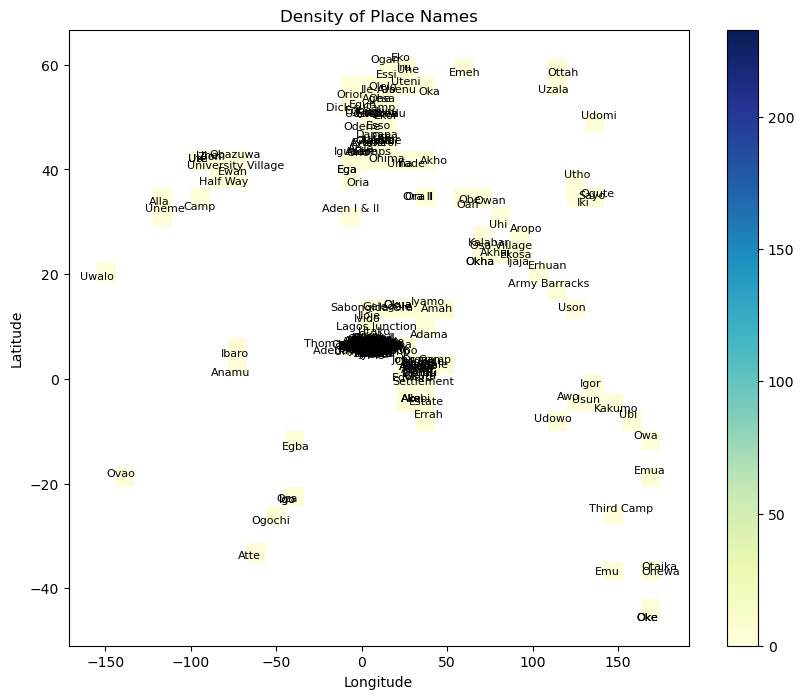
\includegraphics[width=.8\linewidth]{heatmap1.png}
    \caption{Heat map presenting the density of place names}
    \label{fig:heatmap}
\end{figure}


The temporal distribution histogram (Figure~\ref{fig:histgram}) provides insight into the frequency of place names across various historical epochs. The dataset is organized into distinct temporal periods, with each bar representing the count of place names associated with a particular timeframe. By analyzing the distribution of bars, temporal patterns and trends in place-naming practices can be discerned, identifying periods of heightened activity or significance in naming places. This visualization provides the historical context of place names, shedding light on the evolution and dynamics of naming conventions over time.
\begin{figure}[htb]
    \centering
    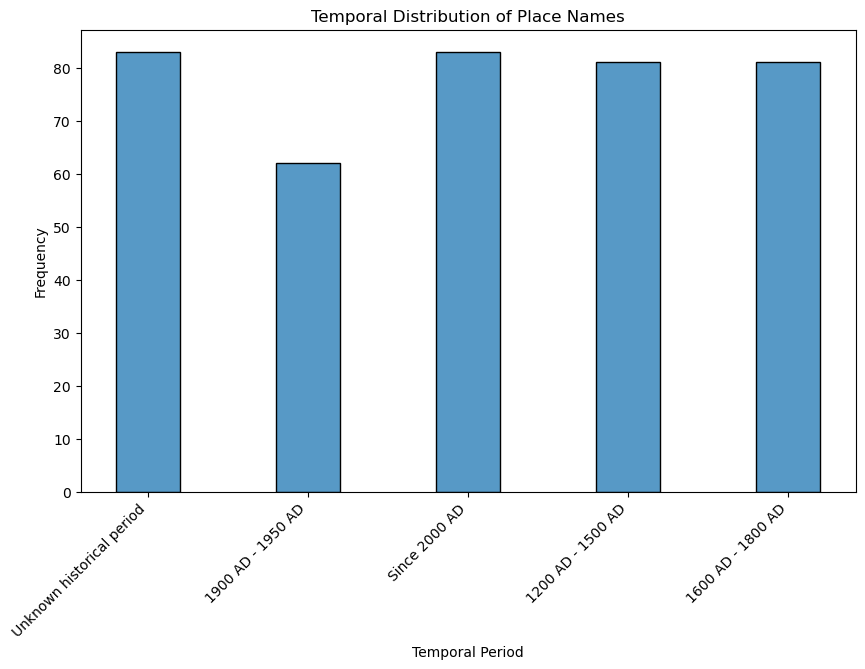
\includegraphics[width=.8\linewidth]{output2.png}
    \caption{Temporal Distribution of Place Names}
    \label{fig:histgram}
\end{figure}

The histogram (Figure~\ref{fig:histogram2}) shows the top 20 most prevalent village names and their frequency in the dataset. It provides a quick insight into common naming trends by displaying the frequency and distribution of village names in the dataset.
\begin{figure}[htb]
    \centering
    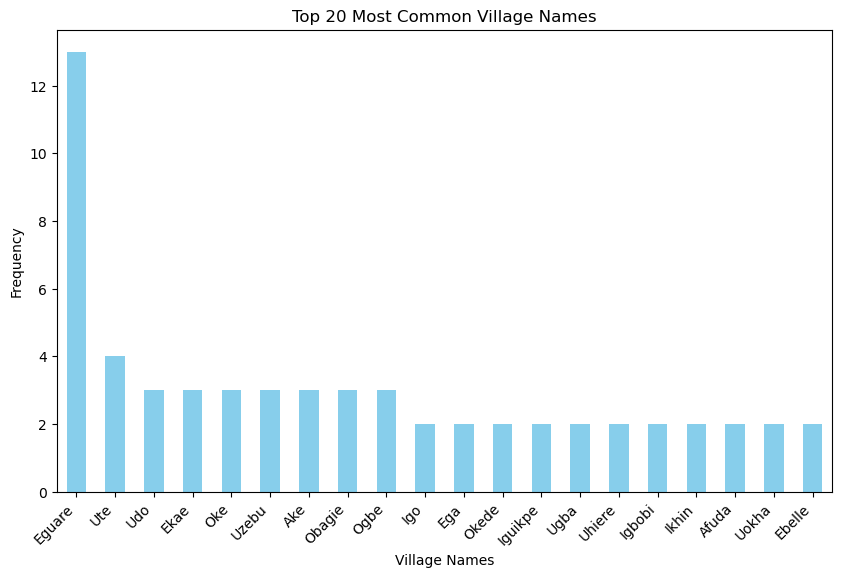
\includegraphics[width=.9\linewidth]{histogram2.png}
    \caption{Top 20 Most Common Village Names}
    \label{fig:histogram2}
\end{figure}





The spatial relationships between place names, depicted in Figure~\ref{fig:network}, were generated using a Python script. This network visualization helps explore the connectivity and relationships between place names based on proximity or connectivity. This can be useful in further research to understand the social or cultural networks that influenced naming practices.
\begin{figure}[htb]
    \centering
    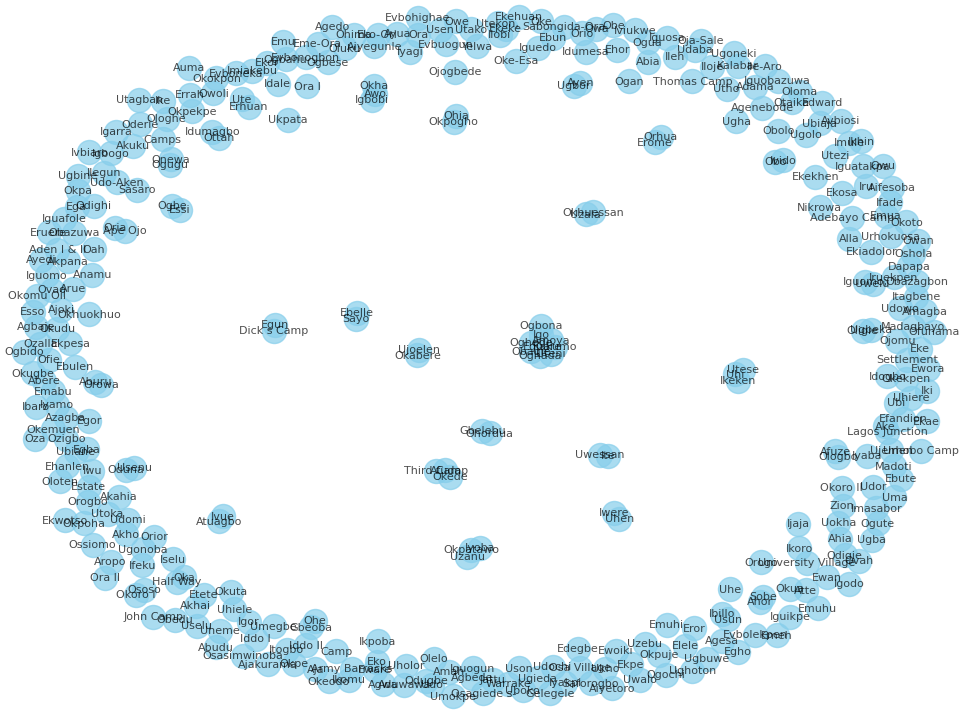
\includegraphics[width=.9\linewidth]{networkanalysis.png}
    \caption{Spatial Relationships between Place Names}
    \label{fig:network}
\end{figure}

The word cloud in Figure~\ref{fig:wordcloud} was also generated using a Python script. This visualization shows the frequency or prevalence of terms in place names, identifying recurring themes or patterns in naming conventions.
\begin{figure}[htb]
    \centering
    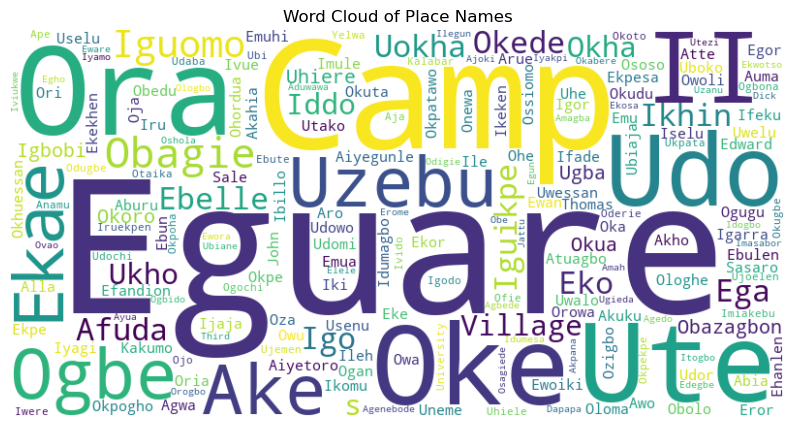
\includegraphics[width=.8\linewidth]{wordcloud.png}
    \caption{Word Cloud of Place Names}
    \label{fig:wordcloud}
\end{figure}

\textbf{Ancient Chronicles:} The investigation of ancient chronicles, such as the "Ife Chronicles" and the "Benin Chronicles," offered foundational accounts of early settlements, legendary narratives, and dynastic histories~\cite{otterbein1966}. According to these chronicles, early settlements were established by legendary figures imbued with divine or semi-divine attributes, signifying their foundational roles in shaping the social and political landscapes of Edo/Benin City. Legendary narratives recount the exploits of these mythical progenitors, depicting their interactions with supernatural beings, the establishment of kinship ties, and the founding of sacred sites. Dynastic histories trace the lineage of ruling families and the succession of kingship within the Edo/Benin polity, highlighting key moments of political consolidation, territorial expansion, and cultural innovation. Through a blend of historical fact and mythic symbolism, these chronicles offer insights into the deep-rooted traditions and cultural heritage underpinning the identity of Edo/Benin City.
\chapter{System Requirements, Design, and Implementation}



\section{Requirements Specification}
The System Requirements Specification (SRS) provides a comprehensive and detailed description of the Place Names Information System (PNIS). It serves as a blueprint for recording data, describing functionalities, and setting performance and design constraints. This SRS ensures a~clear understanding of the system's objectives, requirements, and users' expectations, facilitating a systematic approach to development. This document also helps maintain consistency and ensures that the application meets user needs and thesis goals.

\subsection{Features}
The PNIS connects with a database to store and retrieve information about place names, administrative areas, and other related aspects such as historical data, alternative names, geographical attributes, and user-generated information.
Administrative details provide the foundation for understanding the geographical and administrative context of a place name. The system enhances searchability and discovery by incorporating various names a place name may have, thus improving data accessibility. Geographical features offer a deeper understanding of a place name’s physical characteristics, while historical data enrich place names with stories and events that have occurred over time.

\subsection{Functional Requirements}

\subsubsection{User Management}
Users will be able to register, login, and logout. The application will authenticate users based on securely stored usernames and passwords and will implement mechanisms to reset forgotten passwords. An admin user type will exist with elevated privileges.


\subsubsection{Place Name Management}
Users will be able to search for place names based on various criteria such as name and postal code. The application will display details of a place name including its description, founding year, geographical features, historical events, and alternative names with voice recordings to help with pronunciation. Only authorized users will be allowed to add new place names. They should declare all details for a new place to ensure consistency.

\subsubsection{Content Management}
Users will be able to create and submit posts related to place names. The system will implement a workflow for administrators to approve or reject posts. Users will be able to view posts associated with specific place names and add comments to existing posts.

\subsubsection{Administrative Functions}
Admin users will be able to manage user accounts, update administrative details, and potentially manage other aspects of the data.

\subsection{Non-Functional Requirements}

\subsubsection{Performance}
The system shall be capable of handling large volumes of data efficiently. Data retrieval and query processing shall be optimized for responsiveness, and algorithms for data acquisition shall be designed for scalability and performance.

\subsubsection{User Roles and Security}
Access to the system is role-based, providing different levels of access to the information system for users and administrators. Guests can only search and view place name details. Signed-up users can post comments, and add new place names. Administrators have the authority to approve user posts, modifications and suspend users. To ensure confidentiality and integrity, user passwords are encrypted within the system. Additionally, robust measures are in place to prevent unauthorized access and data breaches.

The system supports the following user roles with their specific functions:
\begin{itemize}
    \item \textbf{Guests} -- are greeted with a search bar that enables them to look up place names and access information about geographical features, alternative names with voice recordings, and administrative details in a table format. They are unable to make posts or submit new place names.
\item \textbf{Users} -- register through a registration form and can log in, reset their passwords if forgotten, and share their experiences by creating posts related to a place. They can also add new place names with detailed information. All user-generated content, such as posts and new place names, must be approved by an admin before becoming visible to other users.
\item \textbf{Admins} -- have a separate login form that directs them to a dedicated dashboard. In this dashboard, admins can approve or reject posts and place names, make users inactive or remove them, and see statistics about the data, such as the number of posts created and their associations with place names.
\end{itemize}

\section{Design Specification}
The Place Names Information System (PNIS) is designed to record, manage, and analyze data related to place names and their attributes. The system aims to provide a comprehensive platform for users to explore and learn about various place names in Edo-Benin City. Below is a detailed blueprint of the system architecture, illustrating how the requirements were implemented.

\subsection{System Architecture Overview}
The architecture of PNIS is designed to be modular, scalable, and secure, ensuring that it can efficiently handle large volumes of data and provide a robust user experience. 
The system is divided into several layers, each responsible for specific functions:
\begin{itemize}
\item \textbf{Presentation Layer} -- was developed using HTML, CSS, JavaScript, and AJAX to create a~responsive and user-friendly interface. The front-end application will interact with the back-end services through RESTful APIs.
\item \textbf{Application Layer}  -- uses PHP for server-side processing, handling requests from the front end and interacting with the database. The server will manage user sessions, authenticate users, and process CRUD operations.
\item \textbf{Data Layer} -- a MySQL relational database designed to store and manage all data related to place names, administrative details, user information, and more. The database schema is normalized to reduce redundancy and improve data integrity. Figure~\ref{fig:dataModel} shows the data model designed to hold the collected data records. The meaning of particular tables is as follows.
\begin{figure}[htb]
    \centering
    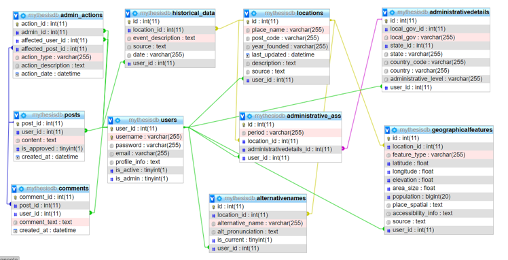
\includegraphics[width=1\linewidth]{model_schema.png}
    \caption{Data Model}
    \label{fig:dataModel}
\end{figure}
The \texttt{administrativedetails} table stores administrative area information such as country, state, and local government. The \texttt{administrative\_ass} table stores associations between administrative areas and specific identifiers (\texttt{location\_id}) during a specific period. The \texttt{admin\_actions} table tracks actions taken by administrators on the system, including affected users or posts. The \texttt{alternativenames} table stores alternative names for locations. The \texttt{comments} table stores information about comments made on posts, including the content and the user who created it. The \texttt{geographicalfeatures} table stores geographical features associated with locations, including type, location data, and descriptions. The \texttt{historical\_data} table stores historical data and events related to locations, including event descriptions, sources, and dates. The \texttt{locations} table contains information about specific place names, including name, postal code, founding year, and descriptions. The \texttt{posts} table stores posts created by users, including content, approval status, and creation time. The \texttt{users} table stores information about users, including username, password, email, profile information, and account status.
\item \textbf{Security Layer} -- implements role-based access control (RBAC) to ensure that only authorized users can access specific features. User passwords are securely stored using hashing algorithms. Guests can search and view place name details, users can create posts and add new place names, and admins can manage posts, place names, and user accounts.
\end{itemize}

The system facilitates communication between the front-end application and the database. The designed API support operations for user management, place name management, and content management. The system handles the integration of data from various sources, including public APIs (e.g., OpenStreetMap), manual data entry, and bulk uploads. This module ensures that data is accurately imported and mapped to the database schema.

\subsection{Workflow and Processes}
To illustrate the workflow and processes within the PNIS, a BPMN (Business Process Model and Notation) diagram is used. This diagram provides a visual representation of the interactions between different user roles (guests, users, admins) and the system functions.
\begin{figure}[htb]
    \centering
    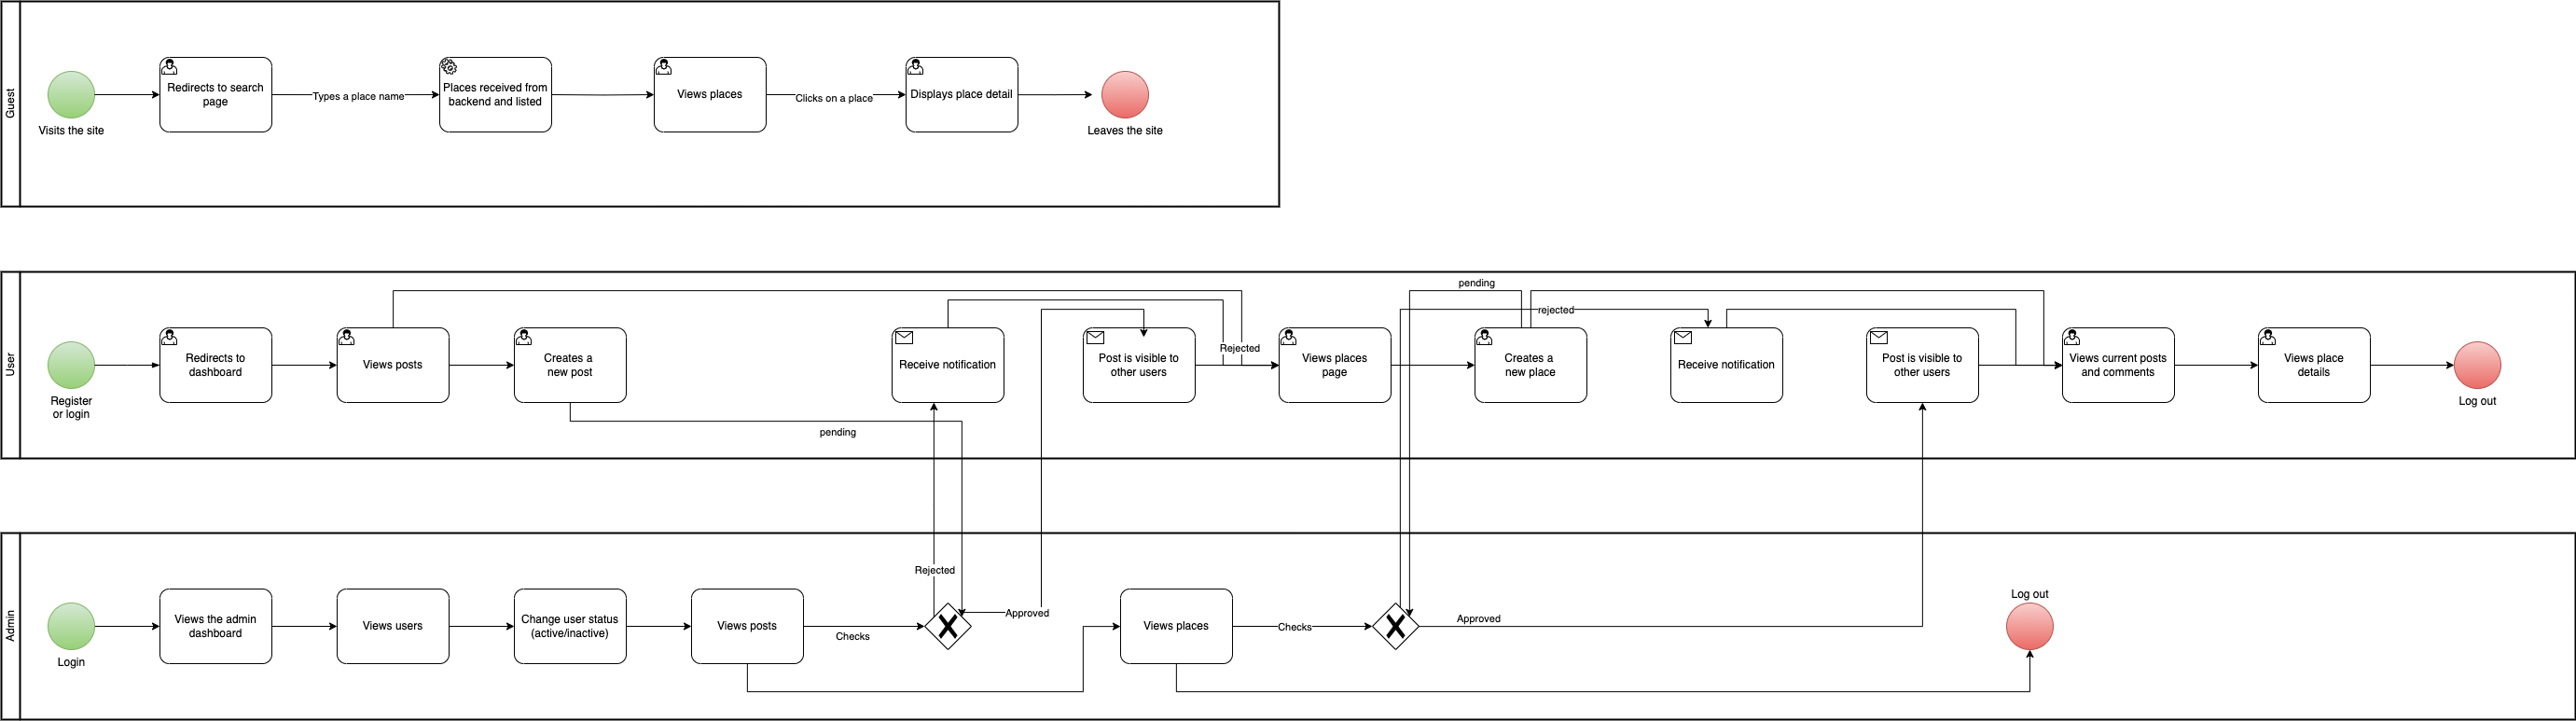
\includegraphics[width=.9\textwidth, keepaspectratio]{bpmn.png}
    \caption{BPMN Diagram for Place Names Information System}
    \label{fig:bpmn}
\end{figure}

The BPMN diagram depicts the following key processes:
\begin{itemize}
    \item \textbf{Guests}: Guests visit the site, search for place names, and view place details.
    \item \textbf{Users}: Users register or log in, create new posts and place names, view posts and place details, and receive notifications about the approval status of their contributions.
    \item \textbf{Admins}: Admins log in to a dedicated dashboard, manage user statuses, approve or reject posts and place names, and view system statistics.
\end{itemize}

These roles and processes ensure that the PNIS operates smoothly, providing an interactive and secure platform for managing and exploring place names.
\subsubsection{User Management}
The system provides a robust user management framework that allows users to register, log in, and manage their accounts. During registration, users can create an account by providing a username, email, and password. The system validates these inputs and securely stores the credentials. Upon successful registration, users gain access to their accounts through the login feature. Additionally, the system includes mechanisms for password management, enabling users to reset forgotten passwords securely via email verification and token-based authentication. Admin users are equipped with elevated privileges, allowing them to manage user accounts, review content, and perform other administrative tasks efficiently.

\subsubsection{Place Name Management}
The place name management functionality enables users to search for and discover place names using various criteria, such as name, postal code, and alternative names. The search functionality is optimized for quick data retrieval, ensuring users can find relevant information promptly. Detailed information about each place name, including its description, founding year, and alternative names, is displayed. Authorized users have the capability to add new place names, complete with relevant details, ensuring the database remains comprehensive and up-to-date.

\subsubsection{Content Management}
The content management system allows users to create and submit posts related to specific place names. These posts can include descriptions, historical data, and personal experiences, enriching the dataset with diverse perspectives. An approval workflow is implemented, whereby administrators review submitted posts and approve or reject them based on predefined criteria. Thus only relevant and accurate content is published. Additionally, users can comment on posts, fostering community interaction and engagement. Comments are moderated to maintain quality and relevance, ensuring the platform remains a valuable resource for all users.

\subsubsection{Administrative Functions}
Administrative functions are designed to provide comprehensive control over the system's data and user interactions. Admin users can manage user accounts, including activating or deactivating accounts and updating user information as needed. Data management capabilities allow administrators to update administrative details, manage place names, and oversee the overall data integrity. This ensures that the system remains accurate, reliable, and useful for all stakeholders.


\section{Implementation of Place Names Information System}
The implementation of the Place Names Information System (PNIS) transforms the design specifications into a functional system. This process encompasses coding various components to ensure they work together seamlessly to meet the specified requirements. The following sections provide a detailed discussion on how the system was implemented.

\subsection{Front-End Development}
The front-end development focused on creating a responsive and user-friendly interface, enabling users to interact with the system efficiently. HTML and CSS were employed for structuring and styling the web pages, ensuring a consistent and visually appealing design. JavaScript and AJAX were used to handle asynchronous requests, enhancing user experience by dynamically updating content without requiring full page reloads.

A key feature of the front end is the search bar, allowing users to search for place names using various criteria such as name, postal code, and alternative names. AJAX calls were utilized to fetch and display real-time search results, ensuring a seamless and interactive user experience.

\subsection{Back-End Development}
The back-end development was implemented using PHP, which handles server-side processing, including user authentication, data processing, and interaction with the database. RESTful APIs were set up to facilitate communication between the front-end application and the database. These APIs manage CRUD (Create, Read, Update, Delete) operations for user management, place name management, and content management.

MySQL was chosen as the relational database management system (RDBMS). The database schema was designed to capture relationships between different entities, ensuring data normalization and integrity. SQL queries and stored procedures were developed to efficiently retrieve and manipulate data based on user inputs and actions.

\subsection{Data Acquisition and Integration}
The system integrates with public APIs, such as OpenStreetMap, to fetch place data. Custom APIs were developed to connect with external data sources, ensuring data is retrieved in a structured and consistent format. User-friendly interfaces for manual data entry were also developed, allowing the enrichment of the database with user entries under specified standards.

Bulk upload capabilities were enabled, allowing the import of data files (e.g., CSV, Excel) from trusted sources. Data mapping techniques were used to align imported data with the database schema, ensuring proper field matching and type conversion.

\subsection{Data Preprocessing and Storage}
To ensure data quality, form validations, and manual review processes were implemented to identify and merge duplicate records, handle missing values, and correct errors. Techniques such as imputation and normalization were used to maintain data integrity.

Data was normalized to fit the relational database schema, ensuring each piece of data is stored in the appropriate table and field. New features were created from raw data to enhance the database, such as calculating population density from area size and population data. Data from multiple sources was merged, resolving conflicts and discrepancies through predefined rules and priority settings. Schema mapping was employed to align data from different sources with the existing database schema.

\subsection{Security Implementation}
Robust security measures were implemented to protect user data and system integrity. Role-based access control (RBAC) ensures that only authorized users can perform specific actions. PHP's built-in cryptography extension was used for password hashing, securely storing user passwords. Additionally, users are provided with mechanisms to reset forgotten passwords securely through email verification and token-based authentication.

In conclusion, the implementation of the Place Names Information System (PNIS) involved meticulous planning and execution across multiple development stages. From front-end and back-end development to data acquisition, preprocessing, and security implementation, each component was carefully crafted to ensure a comprehensive, reliable, and user-friendly system.
% BIBLIOGRAPHY (will be generated automatically)
%NOTE: You must prepare the references' library yourself. A good tool for this is JabRef.
% JabRef, however, offers more record types than BibTeX supports.
% Please do not declare records of types not supported by BibTeX.
% The list of references and citations is formatted in accordance with the declared style.
% Styles that produce numeric citations (in the form [1], [2,3]) are recommended.
% Such a style is, for example, plabbrv
\bibliographystyle{abbrv}
% To control spacing in the literature list, you can use the following command
\setlength{\bibitemsep}{2pt} % - narrows the list
% The bibliography items appears in the table of contents slightly differently than lists of figures, tables, etc.
% To maintain the correct spacing, use the following command
%\addtocontents{toc}{\addvspace{2pt}} % we set the space in the table of contents before the Literature item
% The file name of the prepared library is entered without the .bib extension
% (the line below loads records from the file "bibliography.bib")
\bibliography{bibliography}

\appendix
\chapter{Appendix title}
Lorem ipsum dolor sit amet, consectetur adipiscing elit, sed do eiusmod tempor incididunt ut labore et dolore magna aliqua. Ut enim ad minim veniam, quis nostrud exercitation ullamco laboris nisi ut aliquip ex ea commodo consequat. Duis aute irure dolor in reprehenderit in voluptate velit esse cillum dolore eu fugiat nulla pariatur. Excepteur sint occaecat cupidatat non proident, sunt in culpa qui officia deserunt mollit anim id est laborum.
%\include{appendixB}

% If an index appears in your work, uncomment the following lines
%%\chapterstyle{noNumbered}
%%\phantomsection % sets an anchor
%%\addcontentsline{toc}{chapter}{Index}
%%\printindex

\end{document}




